\chapter{Virtual Organizations}\label{chap:VirtualOrganizations}
As it has been pointed out in the introduction, Magentix2 platform not only has as aims to provide a guaranteed communication mechanism to the programmer, but also to provide a complete support for virtual organizations and SOA-like services. \textsc{Thomas} (Methods, Techniques and Tools for Open Multi-Agent Systems) framework has been integrated with Magentx2 with this purpose \cite{Argente2011}.

%==================================================================
%================== PRIMERA SECCI�N ===============================
%==================================================================
\section{Overview of \textsc{Thomas} framework}

The \textsc{Thomas} framework tries to communicate agents and SOA-like services in a transparent, but independent way.  Agents can offer and invoke services in a transparent way to other agents or entities, as well as external entities can interact with our agents through the use of the offered services.

%\textsc{Thomas} can coexist within different organizational unit, and each organizational unit is composed of agents or other units. In addition, \textsc{Thomas} framework gives us a new communication mechanism consisting of mass communication among agents of the unit taking into account the shipping and receiving of messages by the agents come restricted according to the position that the agent has in the unit. This position is given by the roles playing the agent in the unit.

Different types of virtual organizations are supported by the \textsc{Thomas} framework. Each organization can contain others organizations. Furthermore, diverse roles can be assigned to each organization. These roles are characterized by some attributes which restrict its behavior regarding \textsc{Thomas} framework. Thus, agent must play those roles in order to belong to an organization.

In addition, Magentix2 offers a new communication mechanism based on the virtual organizations structure. Thus, this organizational messaging allows mass communication among agents of an organization, taking into account the type of roles agents play.

\textsc{Thomas} framework consists of a set of modular services. Agents have access to the infrastructure offered by \textsc{Thomas} through a set of services provided by two main agents:

\begin{description}
	\item [Service Facilitator (SF)] This agent offers a yellow page service and also a service descriptor in charge of providing a green page service.
	\item [Organization Manager Service (OMS)] It is mainly responsible of the management of the organizations and their entities. Thus, it allows the creation and the management of any organization and the roles the agents play.
\end{description}

\subsection{Roles in \textsc{Thomas}}\label{sec:ThomasRoles}

Roles  in \textsc{Thomas} are defined with a \textit{RoleName} that acts as an identifier. Furthermore, each role is always associated with a particular organizational unit. Also, each role has the following attributes: $<Position, Accessibility, Visibility>$.

\begin{itemize}
\item \textbf{Position}. The possible values that this field can take are: \textit{Member}, \textit{Supervisor}, \textit{subordinate} or \textit{Creator}.
\begin{itemize}
\item This value must be assigned to roles when they are created.
\item Not all the values are allowed to any type of organization (see section \ref{sec:unitsinthomas}).
\item Anytime an agent registers an organization, it is automatically assigned a new role with a creator position to him. This position gives permission to register and deregister organizations and roles. In addition, it is possible to assign a \textit{creator} role using the services offered by the \textsc{Thomas} API (see section \ref{thomasAPI}).
\end{itemize}

In Table \ref{tab:Role_position} a summary of the role behavior taking into account its position is shown.


\item \textbf{Accessibility}. This attribute allows controlling who can acquire roles. Specifically, the permitted values are:
\begin{itemize}
	\item External: roles can be acquired by agents who do not play any role in the organization.
	\item Internal: in this case, it is necessary participate into the organization, that is, the requested agent should play some role  in the organization.
\end{itemize}


\item \textbf{Visibility}. By means of this attribute it is possible to control what information about roles is provided. Concretely, the allowed values for this attribute are:
\begin{itemize}
\item Public: information services always provide the requested information.
\item Private: the requested information is provided only if the requested  agent belongs to the same organization where the role is registered.
\end{itemize}

\end{itemize}

 The relationship between accessibility and visibility attributes  can be seen in the table \ref{tab:Role_visibility_accessibility}.


\begin{table}[!ht]
\begin{tabular}{|c| c|p{11cm}|}
\hline
\textbf{Position} & Unit Types & \textbf{  Behavior Allowed } \\ \hline
\textit{Creator} & All types& - Send organizational messages is not allowed \\
 && - Register/Deregister units and roles\\
 && - Allocate/Deallocate  roles to other agents\\
 && - Change the hierarchical relations between organizations\\
 && - Acquire other roles\\
 && - Request information about the roles played by other agents\\
 && - Request information about organizations and its elements\\ \hline
\textit{Member} &Flat& - Send organizational messages. These messages will be received for all organization members\\
 &Team& - Register/deregister roles\\
 && - Allocate/deallocate roles to other agents\\
 && - Acquire another role\\
 && - Request information about the roles played by other agents\\
 && - Request information about organizations and its elements\\ \hline
\textit{Supervisor} & Hierarchy&- Send organizational messages. These messages will be received for all organization members\\
&& - Register/Deregister units and roles\\
 && - Allocate/Deallocate  roles to other agents\\
 && - Change the hierarchical relations between organizations\\
 && - Acquire other roles\\
&& - Request information about the roles played by other agents\\
 && - Request information about organizations and its elements\\ \hline
\textit{Subordinate} &Hierarchy&  - Send organizational messages. These messages will be received for all supervisor agents of the organization\\

 && - Acquire other roles\\
&& - Request information about the roles played by other agents\\
 && - Request information about organizations and its elements\\ \hline
 \end{tabular}
\caption{Agent behavior depending of its position}
\label{tab:Role_position}
\end{table}


\begin{table}[!ht]
\begin{tabular}{|c|c|p{11cm}|}
\hline
\textbf{Visibility} & \textbf{Accessibility} & \textbf{Behavior} \\ \hline

\textit{Public} & \textit{External} & Role fully accessible and transparent. The role is visible throughout the system:\\
& & -\textit{External}: any agent can acquire this role \\
& & -\textit{Public}: any agent can request information about the role  \\ \hline

\textit{Public} & \textit{Internal} & Role with restricted access, although visible throughout the system:\\
& & -\textit{Internal}: in order to acquire this role, agents must participate in the organization in which the role was registered(or in its Parent Organization)\\
& & -\textit{Public}: any agent can request information about the role \\ \hline

\textit{Private} & \textit{External} & Role fully accessible, but with limited visibility: \\
& & -\textit{External}: any agent can acquire this role \\
& & -\textit{Private}: information about the role is only provided if requested agents participate in the organization in which the role was registered(or in its Parent Organization). \\ \hline

\textit{Private} & \textit{Internal} & Maximum protection of the role. The unit acts like a black box for these roles:\\
& & -\textit{Internal}: agents must participate in the organization or in its parent organization to acquire the role \\
& & -\textit{Private}: agents can request information about the role if they participate in the organization in which the role was registered(or in its Parent Organization). \\ \hline
\end{tabular}
\caption{How visibility and accessibility attributes affect roles}
\label{tab:Role_visibility_accessibility}
\end{table}


\subsection{Units in \textsc{Thomas}} \label{sec:unitsinthomas}

\textsc{Thomas} framework gives support for three types of organizations or units: \textit{Flat}, \textit{Team} and \textit{Hierarchy}. Each type of organization is governed by different structural norms. In the Table \ref{tab:units} a comparative of these types of units is shown.

Furthermore, there is an organization created by default named \textit{Virtual}. This is a flat unit which represents the \textsc{Thomas} world, and it is the starting point to enter in the system. A role named \textit{Participant} is always available in the \textit{Virtual} organization. This role has the following attributes:

 $<RoleName = Participant, Position = Creator, Visibility = Public, Accessibility = External>$




%\begin{sidewaystable}
\begin{table}
\footnotesize
\begin{center}
\begin{tabular}{|p{3cm}|p{3cm}|p{3cm}|p{5.5cm}|}

\hline
& \textbf{FLAT} & \textbf{TEAM} & \textbf{HIERARCHY} \\ \hline

Allowed role  & \multicolumn{2}{|p{6cm}|}{Creator}  & Creator  \\
positions     & \multicolumn{2}{|p{6cm}|}{Member} & Supervisor  \\
                  & \multicolumn{2}{|p{6cm}|}{}        & Subordinate     \\ \hline

What agents can send organizational messages? &\multicolumn{3}{|p{11.5cm}|}{Any agent from this organization, except those who only play roles with \textit{Position = Creator}} \\ \hline

What agents can receive organizational messages? & \multicolumn{2}{|p{6cm}|}{Any agent from this  organization, except who what only play roles with Position = Creator} & \textit{Supervisors} receive all messages. \textit{Subordinates} only receive messages sent by \textit{Supervisors}. \textit{Creators} do not receive messages.  \\ \hline

What agents can register/deregister organizations? & \multicolumn{3}{|p{11.5cm}|}{Any agent from this  organization which plays roles with \textit{Position = Creator}} \\ \hline

What agents can join an organization to another? & \multicolumn{3}{|p{11.5cm}|}{Any agent from this organization which plays both a role with Position = Creator and  a role with Position = Creator in the new Parent organization.}\\ \hline

What agents can register/deregister roles? & \multirow{2}{3cm}{Any agent from this organization. \textit{Creator} Agents from other organizations } & \multirow{2}{3cm}{Any agent from this organization}. & \multirow{2}{5.5cm}{Agents from this organization with \textit{Position = Creator} or \textit{Position = Supervisor}}. \\ \cline{1-1}

What agents can allocate/deallocate roles? & & & \\
 & & & \\ \hline

What agents can request "public" information? & \multicolumn{3}{|p{11.5cm}|}{Any agent from any organization.}\\ \hline
What agents can request "private" information? & \multicolumn{3}{|p{11.5cm}|}{Any agent from this organization.}\\ \hline
What agents can request information about organizations? & \multirow{2}{3cm}{Any agent from any organization.} & \multicolumn{2}{|p{6cm}|}{\multirow{2}{*}{Any agent from this organization  or any agent from its parent unit.}} \\ \cline{1-1}
What agents can request information about attributes of the roles? & & \multicolumn{2}{|p{6cm}|}{\multirow{2}{*}{}}  \\ \hline
What agents  can acquire roles with accessibility = external?& \multicolumn{2}{|p{6cm}|}{Any agent from any organization.}  & Any agent from any organization. But, it is not allowed to acquire a role with \textit{Position = Creator} or \textit{Position = Supervisor} if the agent already plays a role with Position = Subordinate in the organization.\\ \hline
What agents  can acquire roles with accessibility = internal in the organization? & \multicolumn{2}{|p{6cm}|}{Any agent from this organization  or any agent from its parent unit}  & Any agent from this organization  or any agent from its parent unit.  But, it is not allowed to acquire a role with \textit{Position = Creator} or \textit{Position = Supervisor} if the agent already plays a role with Position = Subordinate in the organization. \\ \hline
\end{tabular}
\caption{Differences among the diverse organization types}
\label{tab:units}
\end{center}
%\end{sidewaystable}
\end{table}
\clearemptydoublepage
\subsection{Service Facilitator}
The SF is a support mechanism  used by organizations and agents to offer and discover services. The SF provides an environment in which the autonomous entities can register service descriptions as directory entries.

%The SF acts as a gateway to access the \textsc{Thomas} platform. The SF can find services searching for a given service profile or searching by the goals that can be fulfilled executing the service. This is done using the matchmaking and service composition mechanisms that are provided by the SF.

The SF acts as a gateway to access the \textsc{Thomas} framework. The SF can find services searching for a given service profile. This is done using matchmaking mechanisms over the inputs, outputs and keywords of the services to search.

The SF also acts as a yellow pages manager and, in this way, it can also find which entities provide a given service. Services may have some pre-conditions that have to be true before the service can be executed. They exchange one or more input and output messages. A successful service execution has some effects on its environment. This parameters are called IOPE (input/output/preconditions/effects). Moreover, there could be additional parameters, which are independent of the service functionality (non-functional parameters), such as quality of service, deadlines, and security protocols among others.


A service represents an interaction between two entities, which are modelled as communications among independent processes. In our case, the Multi-agent Technology provides us with FIPA communication protocols.

Taking into account that we are dealing with semantic services, another important data is the ontology used in the service. When the service description is accessed, any entity has all the needed information available to interact with the service.

Services registered and discovered by SF in \textsc{Thomas} are demanded or offered by some agent or organization (Figure \ref{fig:handledServices}). Demanded services are services which are wished by autonomous entities, but no agent or organization provides them. Offered services are provided and registered in the \textsc{Thomas} environment by agents or organizations. The final execution of this services will be finally made by a web service, an internal behavior of an agent or an agent internal call to a web service.

\begin{figure}[h!t]
	\centering
	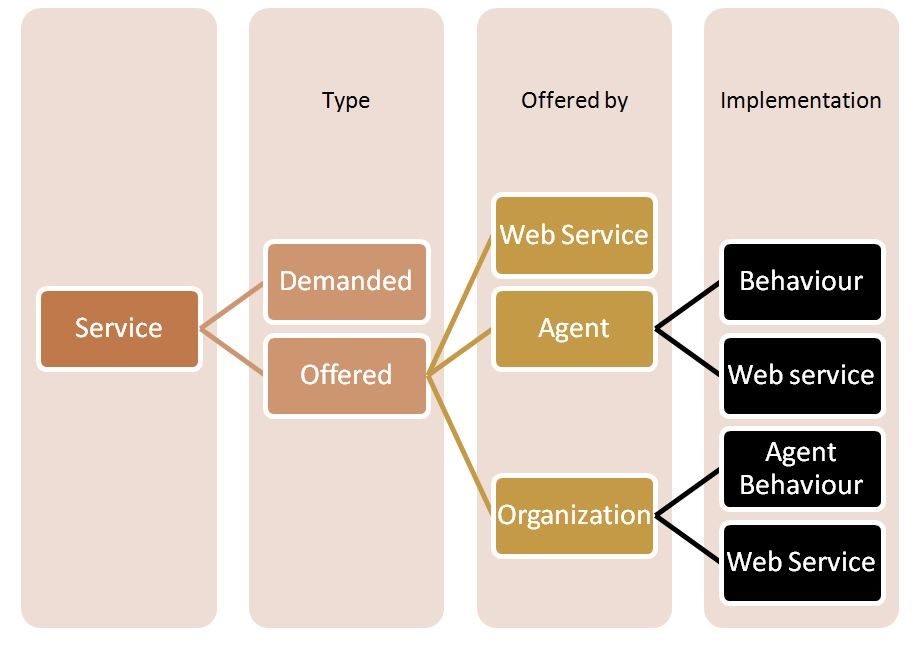
\includegraphics[width=.8\textwidth]{Thomas/images/handledServices.jpg}
	\caption{Handled Services: demanded and implementations of offered services supported}
	\label{fig:handledServices}
\end{figure}


The set of services provided by the SF to manage the services of the platform (meta-services) are classified in 3 categories (these services are described in more detail at Table \ref{tab:thomas_sf_services}):

\begin{itemize}
	\item \textbf{Registration:} they allow adding and removing services from the SF directory.
	\item \textbf{Affordability:} they allow managing the association between providers and their services.
	\item \textbf{Discovery:} services in charge of searching and composing services as an answer to user requirements.
\end{itemize}



\subsection{Organization Manager Service}
This component is in charge of organizations life cycle management, including specification and administration of their structural components (roles, organizative and units) and their execution components (participant agents and the roles they play; and active units in each moment).

The OMS provides agents with a set of services for organization life-cycle management (\cite{DelVal09}), classified in:

\begin{itemize}
	\item \textbf{Structural services:} which modify the structural organization specification, i.e. roles, organizational units and norms (see Table \ref{tab:thomas_OMSProxy_registration}).
	\item \textbf{Informative services:} that give information of the current state of the organization (see Table \ref{tab:thomas_OMSProxy_information}).
	\item \textbf{Dynamic services:} that allow managing role enactment and dynamic entry/exit of agents (see Table \ref{tab:thomas_OMSProxy_compound}).
\end{itemize}

These services are  published in the SF and also available thought the OMSproxy class (see section \ref{sec:programmingAgentsThomas}).


\subsection{Normative Context}

As we explain in sections \ref{sec:ThomasRoles} and \ref{sec:unitsinthomas}, there are some predefined norms (called structural norms) which control the access to OMS services. Thus, some OMS services are only available if  agents which request them play some role inside the organization with a concrete position (table \ref{tab:rol_acces}). It is possible to avoid these structural norms or make them more restrictive by means of defining new norms using the \textit{registerNorm} service of the OMS. In this way, users can add \textsc{Permitted} or \textsc{Forbidden}  norms to relax or restrict  the access control to the OMS services in an organization. 


\begin{table}[h!t]
\centering
\begin{tabular} {|l | c c c c | }
\hline
&\multicolumn{4}{c |}{Position}\\
OMS Services & Creator & Member & Supervisor & Subordinate \\
\hline
RegisterUnit & x & - & - & -\\
DeregisterUnit & x & - & - & -\\
RegisterRole & x & x & x & -\\
DeregisterRole & x & x & x & -\\
RegisterNorm & x & x & x & -\\
DeregisterNorm & x & x & x & -\\
AquiereRole & x & x & x &x \scriptsize{(2)} \\
LeaveRole & x & x & x &x  \\
AllocateRole & x & x & x & -\\
DeallocateRole & x & x & x & -\\
JointUnit & x \scriptsize{(1)} & - &-&-\\
InformAgentRole  & x & x & x &x  \\
InformMembers & x & x & x &x  \\
InformQuantityMembers & x & x & x &x  \\
InformUnit & x & x & x &x  \\
InformUnitRoles & x & x & x &x  \\
InformTargetNorms & x & x & x &x  \\
InformRole & x & x & x &x  \\
InformNorm & x & x & x &x  \\
\hline
\multicolumn{5}{| l |}{\scriptsize{(1) The agent should also play another role with position=creator in the parent unit}}\\
\multicolumn{5}{| l |}{\scriptsize{(2) The agent could acquire another role with posistio=creator or position=supervisor in its organization}}\\
\hline

\end{tabular}
\caption{OMS Proxy: Service Access taking into account the role position played by the requesting agent}
\label{tab:rol_acces}
\end{table}

\subsubsection{Norm Description}
Norms are registered into an organizational unit with a unique name inside that organization. They should be written following the syntax of the \textsc{Thomas} normative language (see appendix \ref{app:BNFSyntax} for a detailed explanation), which is based on AgentSpeak language. Concretely, the appearance of a norm is as follows : \\
$$@normName[Deontic, Target, Action, Activation, Expiration]$$
where:

\begin{itemize}
 \item $Deontic \in \lbrace f,o,p \rbrace$ , where $f$ is used for forbidden norms, which restrict the access to services; $o$ is used for obligation norms; and $p$ is used for permitted norms, which relax the access to services. Although a norm can be registered with a deontic value  of obligation, the OMS only manage forbidden or permitted norms. 	
 \item $Target=<type,id>$ where $type \in   \lbrace agentName, roleName, positionName \rbrace $, whereas $id$ is the associated value (for example, the position value \textit{creator}) or the anonymous variable ``\_'' (when any value is accepted).  The field \textit{target} allows users to determine which agents will be affected by a norm. For example, taking into account an scenario in which a norm was registered in a unit with the target $<agentName, consumer>$, this norm only affects the agent which name is \textit{consumer}. 
 
 \item $Action$ is the name of the service. \textsc{Thomas} only manage norms which action correspond with an OMS service (see appendix \ref{app:BNFSyntax} to build Action field correctly).
 
 \item $Activation$ is a well-formed formula expressed by means of first-order predicates which indicates the conditions to fulfil a norm. Until a service is provided, the OMS agent checks if some norm is satisfied, in which case that norm is applied. Users should add predicates related with data known in the \textsc{Thomas} world, such as role details, played roles , organization structure, agent names, etc (see \ref{app:BNFSyntax} for further explanation). The \textit{Activation}  could be empty (``\_'' ), in that case the norm is always fulfilled.
 
 \item  $Expiration$ is a well-formed formula expressed by means of first-order predicates which indicates when a norm expires. So, if the expiration of a norm is satisfied, the norm is not applied although the activation is fulfilled. Users should add predicates related with data known in the \textsc{Thomas} world, such as role details, played roles , organization structure, agent names, etc (see \ref{app:BNFSyntax} for further explanation). The  \textit{Expiration} could be empty (``\_'' ), in that case the norm never expires.
 
\end{itemize}

\subsubsection{Norm Checking}

The OMS agent is the responsible of verifying if some norm applies before provide a service. Thus, users can add forbidden or permitted norms to restrict or relax the predefined rules for accessing to services,  respectively. In particular, the order in which the restrictions and norms are checked before provide a service of the OMS is as follows: 
\begin{enumerate}
\item \textit{\textsc{Permitted} norms.} It is checked if there are some permitted norms registered which action correspond with the requested service. In that case, it is also checked if those norms are fulfilled, that is, their target and activations are satisfied whereas their expiration are not. In case a permitted norm is satisfied, the service is provided with no restrictions and  no structural norm related with unit types or role properties are considered. Concretely, the properties of the roles (accessibility, visibility, position) are not taking into account in the execution of the services (such as informative services).

\item \textit{\textsc{Forbidden} norms.}  It is checked if there are some forbidden norms registered which action correspond with the requested service. In that case, it is also checked if those norms are fulfilled, that is, their target and activations are satisfied whereas their expiration are not. If a forbidden norm is satisfied, the service is not provided and a ForbiddenNormException exception is thrown. 

\item \textit{Structural norms.} All predefined norms of the service are checked before provide the service. If no one is satisfied, the service is provided as usual.
\end{enumerate}

\subsubsection{Normative Example: Forum}


\begin{figure}[hbtp]
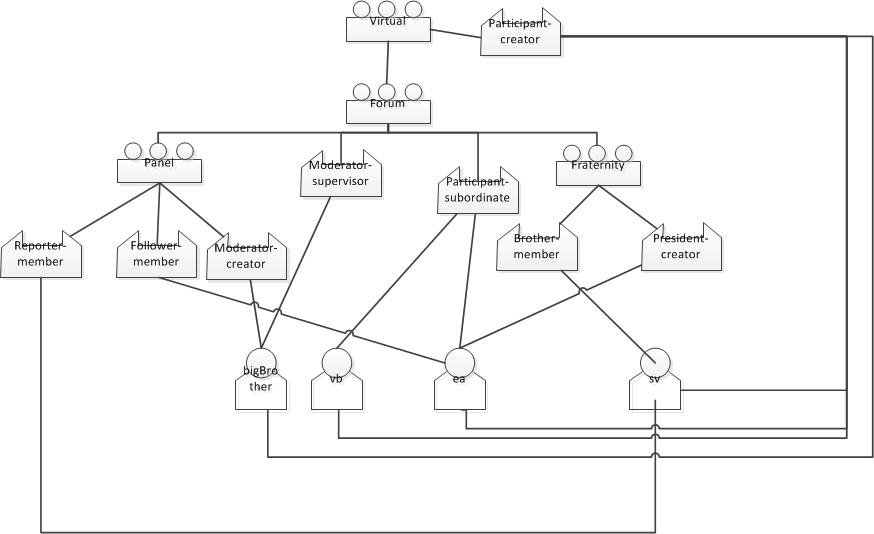
\includegraphics[width=1\textwidth]{Thomas/images/ejemploNormas.jpg}
\caption{Organizational view of the form example: organizations, roles and agents}
\label{fig:normExample}
\end{figure}

In this section,  an example of how to use the normative context provided by \textsc{Thomas} is explained. Concretely,  the Figure \ref{fig:normExample} shows the scenario, where there are three units:  an organization named \textit{forum} (which type is \textit{hierarchy}) and its two descendent organizations \textit{fraternity} (which type is \textit{team}) and \textit{panel} (which type is \textit{flat}). Furthermore, there is the \textit{virtual} unit, which represents the \textsc{Thomas} world  and acts as the starting point to enter in the system, as mentioned before (see section \ref{sec:unitsinthomas}). In the \textit{forum} unit there are the following roles:

\begin{itemize}
\item \textbf{Moderator:} It acts as supervisor and moderator of the forum. Its role attributes are: position=supervisor; accessibility=internal; visibility=private.
\item \textbf{Participant:} It participates in the forum.  Its role attributes are: position=subordinate; accessibility=internal; visibility=public.
\end{itemize}

The \textit{fraternity} unit has two roles:

\begin{itemize}
\item \textbf{President:} It acts as a president of the \textit{fraternity} and it is in  charge of adding/deleting norms and roles.  Only one agent can play this role. Its role attributes are: position=creator; accessibility=internal; visibility=private.
\item \textbf{Brother:} It represents a member of the \textit{fraternity}, in fact, all the participants of the \textit{fraternity} should play this role.  Its role attributes are: position=member; accessibility=external; visibility=public.
\end{itemize}

The \textit{panel} unit has three different roles:
\begin{itemize}
\item \textbf{Moderator:} It should be played by an unique agent which also plays the role \textit{moderator} in the \textit{forum} unit. It is in charge of adding new norms to the unit. It can not add new roles. Its role attributes are: position=creator; accessibility=internal; visibility=private.
\item \textbf{Reporter:} It should be played by agents which add news to the panel. They are not allowed to add norms/roles in the unit. Its role attributes are: position=member; accessibility=external; visibility=private.
\item \textbf{Follower:} It should be played by agents which read news from the panel.  They are not allowed to add norms/roles in the unit. Its role attributes are: position=member; accessibility=external; visibility=public.
\end{itemize}

Regarding the \textit{forum} unit, creating new roles with position \textit{creator} is not allowed.  Respecting the fraternity unit, creating new roles with position \textit{creator} is prohibited. Concerning the \textit{panel} organization, it is prohibited that agents know which roles are played by other agents. Also, changing the parent unit of the organizations is prohibited.   

Following, some of the norms needed to obey the specification of the forum scenario are described using the \textsc{Thomas} syntax (see appendix \ref{app:BNFSyntax}, section \ref{sec:forumpredicates} in order to know for the predicates  the OMS uses for reasoning):
\begin{itemize}
\item \textbf{Unit \textit{forum}}
\begin{itemize}
\item It is not allowed registering new roles with the position \textit{creator}:
\begin{verbatim}
@noRegRole[ f, <positionName:supervisor>, 
registerRole(_,forum, _, _, creator,_), _ , _ ] 
\end{verbatim}

\item Changing the parent unit of the organization is prohibit.  
\begin{verbatim}
@noJoinUnit[ f, <positionName:_>, 
joinUnit(forum,_,_), _ , _ ] 
\end{verbatim}

\end{itemize}

\item \textbf{Unit \textit{fraternity}}
\begin{itemize}
\item Only one agent can play the role \textit{president}:
\begin{verbatim}
@noAcRolePresident[ f, <agentName:_>, 
acquireRole(president, fraternity, _),
roleCardinality(president,fraternity,1),  _ ] 
\end{verbatim}

\item Only the role \textit{president} can add new norms:
\begin{verbatim}
@noRegNorm[ f, <positionName:member>, 
registerNorm(_, fraternity, _, _),_ ,_ ] 
\end{verbatim}

\item Only the role \textit{president} can delete norms:
\begin{verbatim}
@noDelNorm[ f, <positionName:member>, 
deregisterNorm(_, fraternity, _, _),_ ,_ ] 
\end{verbatim}

\item Only the  \textit{president} can add new roles:
\begin{verbatim}
@noRegRole[ f, < positionName:member>, 
registerRole(_,fraternity, _, _, _,_), _ , _ ] 
\end{verbatim}

\item Only the  \textit{president} can delete roles:
\begin{verbatim}
@noDeRegRole[ f, <positionName:member>,
 deregisterRole(_,fraternity, _), _ , _ ] 
\end{verbatim}

\item It is not allowed registering new roles with the position \textit{creator}:
\begin{verbatim}
@noRegRoleCreator[ f, <agentName:_>, 
registerRole(_,fraternity, _, _, creator,_), _ , _ ] 
\end{verbatim}


\item Changing the parent unit of the organization is prohibit.  
\begin{verbatim}
@noJoinUnit[ f, <positionName:_>, 
joinUnit(fraternity,_,_), _ , _ ] 
\end{verbatim}


\end{itemize}

\item \textbf{Unit \textit{panel}}
\begin{itemize}

\item  Only one agent can play the role \textit{moderator}:
\begin{verbatim}
@noAcRoleModerator[ f, <agentName:_>, 
acquireRole(moderator, panel, _),  
roleCardinality(moderator,panel,1),   _ ]
\end{verbatim}

\item The agent which plays the role \textit{moderator} should play the role \textit{moderator} in the \textit{forum} unit

\begin{verbatim} 
@controlAcRoleModerator[ f, <agentName:_>, 
acquireRole(moderator, panel,  Ag), 
not(playsRole(Ag, moderator, forum)), _ ]
\end{verbatim}

\item Only the role \textit{moderator} can add norms
\begin{verbatim}
@noRegNorm[ f, <agentName:Ag>, 
registerNorm(_, panel, _, Ag),
not playsRole(Ag,moderator, plana),_  ] 
\end{verbatim}

\item Only the role \textit{moderator} can delete norms
\begin{verbatim}
@noDeregNorm[ f, <agentName:Ag>, 
deregisterNorm(_, panel, Ag),
not playsRole(Ag,moderator, plana),_  ] 
\end{verbatim}

\item No one can add roles
\begin{verbatim}
@noRegRole[ f, < positionName:_>, 
registerRole(_,panel, _, _, _,_), _ , _ ] 

@noDeRegNormRegRole[ f, <roleName:moderator>, 
deregisterNorm(NormX, panel, _),
hasAction(NormX,panel, registerRole), _ ] 
\end{verbatim}


\item No one can delete roles
\begin{verbatim}
@noDeRegRole[ f, <positionName:_>, 
deregisterRole(_, panel, _),_, _ ] 

@noDeRegNormDeregRole[ f, <roleName:moderator>, 
deregisterNorm(NormX, panel, _),
hasAction(NormX,panel, deregisterRole), _ ] 
\end{verbatim}

\item Knowing which roles are played by other agents is prohibit
\begin{verbatim}
@noSupInfAgRole[ f, <agentName:Ag>,
informAgentRole(Ag,_), _ , _ ] 

@noDeRegNormnoSupInfAgRole[ f, <roleName:moderator>,
deregisterNorm(NormX, panel, _),
hasAction(NormX,panel, informAgentRole), _ ] 

\end{verbatim}

\item Changing the parent unit of the organization is prohibit.   
\begin{verbatim}
@noJoinUnit[ f, <positionName:_>, 
joinUnit(panel,_,_), _ , _ ] 
\end{verbatim}

\end{itemize}

\end{itemize}


%==================================================================
%================== SEGUNDA SECCI�N ===============================
%==================================================================

\section{Programming agents which use \textsc{Thomas}}\label{sec:programmingAgentsThomas}

\subsection{Magentix2 API for \textsc{Thomas}}\label{thomasAPI}
SF and OMS have been defined as two types of intermediary agents in order to address the translation between Magentix2 agents (or any external agent), that implement FIPA communication,and the services they provide. Services requests through FIPA-request protocol were received by this type of agents.

In order to ease the interaction among user agents and OMS and SF agents, two classes are provided (\lstinline|OMSProxy| and \lstinline|SFProxy|). They work as a proxy for OMS and SF respectively, encapsulating and hiding the details of the underlying communication protocol.Thus, the developer can interact with OMS and SF using simple function calls \footnote{Notice that only Queue and Conversational Agents can make use of these proxy classes, because  the capacity of follow a conversation is required} .

\subsubsection{OMSProxy}

\begin{figure}[h!t]
	\centering
	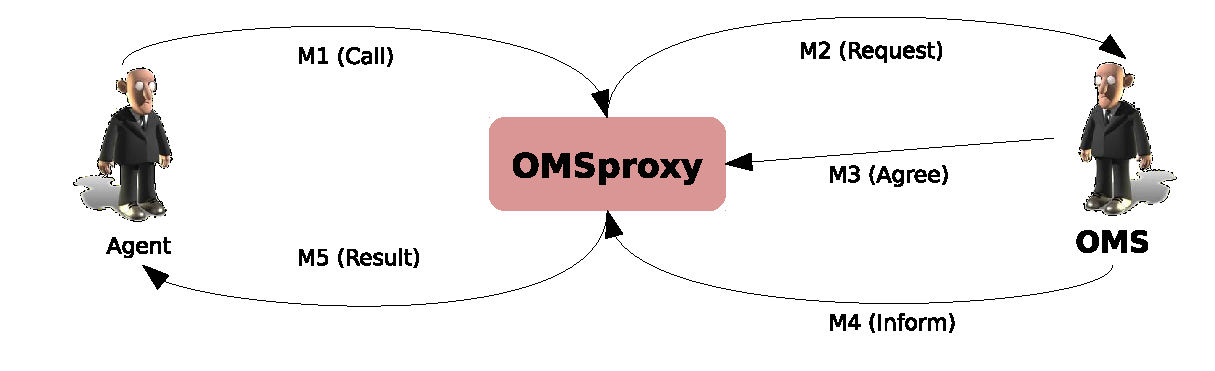
\includegraphics[width=1.0\textwidth]{Thomas/images/oms_omsProxy_interaction}
	\caption{Interaction between user agent and OMS agent through the OMSProxy}
\end{figure}

The OMSProxy can be found in the package \lstinline|es.upv.dsic.gti_ia.organization|. To use its functionality, a new instance of the \lstinline|OMSProxy| class must be created to access the methods contained in the OMS. In the constructor, the agent who executes the service has to be specified. There are two options. In the first one, the url where OMS services are deployed is taken from the \textit{settings.xml} configuration file (please see section \ref{chap:PlatformAdministration}). Notice that this is the recommended option.

\begin{lstlisting}
	private OMSProxy omsProxy = new OMSProxy(this);
\end{lstlisting}

On the contrary, in the second option, the url where OMS services are deployed (.war) should be specified in the constructor if the user does not want to use the default url from the \textit{settings.xml} configuration file:

\begin{lstlisting}
	private OMSProxy omsProxy = new OMSProxy(this, "url");
\end{lstlisting}


OMSProxy provides a developer with a set of methods to manage available services. This services are classified into three different types: structural, dynamic and informative. Tables \ref{tab:thomas_OMSProxy_registration}, \ref{tab:thomas_OMSProxy_information}, \ref{tab:thomas_OMSProxy_compound} and \ref{tab:thomas_OMSProxy_messaging} show respectively these sub-types. These methods return a string if are successfully provided. If not, they through a \textsc{Thomas} exception (see appendix \ref{app:Exceptions} for further details). 

Some OMS services are only available if  agents which request them play a role inside the organization with a determined position. Table \ref{tab:rol_acces} summarizes  the available access to the services taking into account the position of the role.


\begin{longtable}{|p{3cm}|r|p{8.5cm}|}
  \hline
  \multirow{8}{*}{\textbf{RegisterRole}} & Description: & Creates a new role within a unit \\ \cline{2-3}
    & Inputs: & RoleName (Identifier of the new role) \\ \cline{3-3}
    &  & UnitName (Identifier of the organizational unit) \\ \cline{3-3} 
    &  & Accessibility (\texttt{internal} or \texttt{external}) \\ \cline{3-3} 
    &  & Visibility (\texttt{public} or \texttt{private}) \\ \cline{3-3} 
    &  & Position (\texttt{member}, \texttt{supervisor} or \texttt{subordinate}) \\ \cline{2-3}
    & Outputs:     & RoleName + \texttt{created} \\ \cline{2-3}
    & Exceptions:  & InvalidPositionException, ForbiddenNormException, NotSupervisorOrCreatorInUnitException, NotMemberOrCreatorInUnitException, InvalidUnitTypeException, NotInUnitAndNotCreatorException, AgentNotInUnitException, RoleExistsInUnitException, UnitNotExistsException, NotValidIdentifierException, EmptyParametersException \\ \hline
  \hline
  \multirow{5}{*}{\textbf{DeregisterRole}} & Description: & Removes a specific role from a unit \\ \cline{2-3}
    & Inputs: & RoleName (Identifier of the role) \\ \cline{3-3}
    &  & UnitName (Identifier of the unit) \\ \cline{2-3}
    & Outputs:     & RoleName + \texttt{deleted} \\ \cline{2-3}
    & Exceptions:  & ForbiddenNormException, NotSupervisorOrCreatorInUnitException, NotMemberOrCreatorInUnitException, InvalidUnitTypeException, NotInUnitAndNotCreatorException, AgentNotInUnitException, RoleInUseException, RoleContainsNormsException, RoleNotExistsException, UnitNotExistsException, EmptyParametersException \\ \hline
  \hline
  \multirow{7}{*}{\textbf{RegisterUnit}} & Description: & Creates a new unit within a specific organization \\ \cline{2-3}
    & Inputs: & UnitName (Identifier of the new unit) \\ \cline{3-3}
    &  & Type (\texttt{flat}, \texttt{team} or \texttt{hierarchy}) \\ \cline{3-3}
    &  & ParentUnitName (Identifier of the parent unit) \\ \cline{3-3}
    &  & Creator (The name of the new creator role) \\ \cline{2-3}
    & Outputs:     & UnitName + \texttt{created} \\ \cline{2-3}
    & Exceptions   & ParentUnitNotExistsException, ForbiddenNormException, NotCreatorInParentUnitException, UnitExistsException, NotValidIdentifierException, EmptyParametersException \\ \hline
  \hline
  \multirow{4}{*}{\textbf{DeregisterUnit}} & Description: & Removes a unit from an organization \\ \cline{2-3}
    & Inputs: & UnitName (Identifier of the unit) \\ \cline{2-3}
    & Outputs:     & UnitName + \texttt{deleted} \\ \cline{2-3}
    & Exceptions:  & NotCreatorAgentInUnitException, SubunitsInUnitException, ForbiddenNormException, NotCreatorInUnitOrParentUnitException, VirtualUnitException, UnitNotExistsException, EmptyParametersException \\ \hline
  \hline
  \multirow{5}{*}{\textbf{JoinUnit}} & Description: & Updates the parent unit \\ \cline{2-3}
    & Inputs: & UnitName (Identifier of the unit) \\ \cline{3-3}
    &  & ParentUnitName (Identifier of the new parent unit) \\ \cline{2-3}
    & Outputs:     & UnitName + \texttt{joined to} + ParentUnitName \\ \cline{2-3}
    & Exception:   & SameUnitException, VirtualParentException, ForbiddenNormException, NotCreatorInParentUnitException, NotCreatorInUnitException, AgentIDntNotInUnitException, ParentUnitNotExistsException, UnitNotExistsException, EmptyParametersException \\ \hline
  \hline
  \multirow{5}{*}{\textbf{RegisterNorm}} & Description: & Creates a new norm within a specific organization that can be associated to a role, position or agent. \\ \cline{2-3}
    & Inputs: & UnitName (Identifier of the unit) \\ \cline{3-3}
    &  & NormContent (The norm described in THOMAS language, see appendix \ref{app:BNFSyntax}) \\ \cline{2-3}
    & Outputs:     & NormName + \texttt{registered} \\ \cline{2-3}
    & Exceptions:  & RoleNotExistsException, InvalidPositionException, InvalidUnitTypeException, ForbiddenNormException, NotSupervisorOrCreatorInUnitException, NotMemberOrCreatorInUnitException, InvalidUnitTypeException, NotInUnitAndNotCreatorException, AgentNotInUnitException, NormExistsInUnitException, UnitNotExistsException, EmptyParametersException \\ \hline
  \hline
  \multirow{5}{*}{\textbf{DeregisterNorm}} & Description: & Removes a specific norm from a unit \\ \cline{2-3}
    & Inputs: & NormName (Identifier of the norm) \\ \cline{3-3}
    &  & UnitName (Identifier of the unit) \\ \cline{2-3}
    & Outputs:     & NormName + \texttt{deleted} \\ \cline{2-3}
    & Exceptions:  & ForbiddenNormException, NotSupervisorOrCreatorInUnitException, NotMemberOrCreatorInUnitException, InvalidUnitTypeException, NotInUnitAndNotCreatorException, AgentNotInUnitException, NormNotExistsException, UnitNotExistsException, EmptyParametersException \\ \hline
\caption{OMS Proxy: Structural services API}
\label{tab:thomas_OMSProxy_registration}
\end{longtable}

\begin{longtable}{|p{3cm}|r|p{8.5cm}|}
  \hline
  \multirow{5}{*}{\textbf{InformRole}} & Description: & Provides a role description of a specific unit \\ \cline{2-3}
    & Inputs: & RoleName (Identifier of the role) \\ \cline{3-3}
    &  & UnitName (Identifier of the unit) \\ \cline{2-3}
    & Outputs:     & \textless Accessibility, Visibility, Position\textgreater \\ \cline{2-3}
    & Exceptions:  & ForbiddenNormException, VisibilityRoleException, RoleNotExistsException, UnitNotExistsExceptiontsException, EmptyParametersException \\ \hline
  \hline
  \multirow{4}{*}{\textbf{InformUnit}} & Description: & Provides unit description \\ \cline{2-3}
    & Inputs: & UnitName (Identifier of the unit) \\ \cline{2-3}
    & Outputs:     & \textless UnitType, ParentUnitName\textgreater \\ \cline{2-3}
    & Exceptions:  & ForbiddenNormException, NotInUnitOrParentUnitException, InvalidUnitTypeException, UnitNotExistsException, EmptyParametersException \\ \hline
  \hline
  \multirow{4}{*}{\textbf{InformUnitRoles}} & Description: & List the roles that have been registered inside a unit \\ \cline{2-3}
    & Inputs: & UnitName (Identifier of the unit) \\ \cline{2-3}
    & Outputs:     & \textless RoleName, Accessibility, Visibility, Position\textgreater \\ \cline{2-3}
    & Exceptions:  & ForbiddenNormException, UnitNotExistsException, EmptyParametersException \\ \hline
  \hline
  \multirow{4}{*}{\textbf{InformAgentRole}} & Description: & List the roles and units in which an agent is in a specific moment. \\ \cline{2-3}
    & Inputs: & RequestedAgentName (Identifier of the agent requested) \\ \cline{2-3}
    & Outputs:     & \textless RoleName, UnitName\textgreater \\ \cline{2-3}
    & Exceptions:  & AgentNotExistsException, ForbiddenNormException, EmptyParametersException \\ \hline
  \hline
  \multirow{6}{*}{\textbf{InformMembers}} & Description: & Indicates entities that are members of a specific unit. Optionally, it is possible to specify a role and position of this unit, so then only members playing this role or position are detailed \\ \cline{2-3}
    & Inputs: & UnitName (Identifier of the unit) \\ \cline{3-3}
    &  & RoleName (Identifier of the role) \\ \cline{3-3}
    &  & Position (\texttt{member}, \texttt{supervisor} or \texttt{subordinate}) \\ \cline{2-3}
    & Outputs:     & \textless AgentName, RoleName\textgreater \\ \cline{2-3}
    & Exceptions:  & RoleNotExistsException, InvalidRolePositionException, ForbiddenNormException, AgentNotExistsException, UnitNotExistsException, EmptyParametersException \\ \hline
  \hline
  \multirow{6}{*}{\parbox{3cm}{\textbf{InformQuantity- Members}}} & Description: & Provides the number of current members of a specific unit. Optionally, if a role and position is indicated then only the quantity of members playing this roles or position is detailed \\ \cline{2-3}
    & Inputs: & UnitName (Identifier of the unit) \\ \cline{3-3}
    &  & RoleName (Identifier of the role) \\ \cline{3-3}
    &  & Position (\texttt{member}, \texttt{supervisor} or \texttt{subordinate}) \\ \cline{2-3}
    & Outputs:     & Integer \\ \cline{2-3}
    & Exceptions:  & RoleNotExistsException, InvalidRolePositionException, ForbiddenNormException, AgentNotExistsException, UnitNotExistsException, EmptyParametersException \\ \hline
  \hline
  \multirow{5}{*}{\textbf{InformNorm}} & Description: & Provides the content of the norm \\ \cline{2-3}
    & Inputs: & NormName (Identifier of the norm) \\ \cline{3-3}
    &  & UnitName (Identifier of the unit) \\ \cline{2-3}
    & Outputs:     & ContentNorm  \\ \cline{2-3}
    & Exceptions:  & ForbiddenNormException, NotInUnitOrParentUnitException, InvalidUnitTypeException, NormNotExistsException, UnitNotExistsException, EmptyParametersException \\ \hline
  \hline
  \multirow{5}{*}{\parbox{3cm}{\textbf{InformTarget- Norms}}} & Description: & Provides information about a specific norm \\ \cline{2-3}
    & Inputs: & TargetTypeName (\texttt{roleName}, \texttt{positionName} or \texttt{agentName}) \\ \cline{3-3}
    &  & TargetTypeValue (Identifier of the object affected by norm or '\_') \\ \cline{3-3}
    &  & UnitName (Identifier of the unit) \\ \cline{2-3}
    & Outputs:     & \textless NormName, UnitName, TargetTypeName, TargetTypeValue\textgreater \\ \cline{2-3}
    & Exceptions:  & ForbiddenNormException, AgentNotInUnitException, InvalidTargetTypeException, UnitNotExistsException, EmptyParametersException \\ \hline
\caption{OMS Proxy: Informative services API}
\label{tab:thomas_OMSProxy_information}
\end{longtable}


\begin{longtable}{|p{3cm}|r|p{8.5cm}|}
  \hline
  \multirow{5}{*}{\textbf{AcquireRole}} & Description: & Requests the adoption of a specific role within a unit \\ \cline{2-3}
    & Inputs: & RoleName (Identifier of the role) \\ \cline{3-3}
    &  & UnitName (Identifier of the unit) \\ \cline{2-3}
    & Outputs:     & RoleName + \texttt{acquired} \\ \cline{2-3}
    & Exceptions:  & PlayingRoleException, ForbiddenNormException, NotSupervisorOrCreatorInUnitException, NotInUnitOrParentUnitException, RoleNotExistsException, UnitNotExistsException, EmptyParametersException \\ \hline
  \hline
  \multirow{5}{*}{\textbf{LeaveRole}} & Description: & Requests to leave a role \\ \cline{2-3}
    & Inputs: & RoleName (Identifier of the role) \\ \cline{3-3}
    &  & UnitName (Identifier of the unit) \\ \cline{2-3}
    & Outputs:     & RoleName + \texttt{left} \\ \cline{2-3}
    & Exceptions:  & NotPlaysRoleException, ForbiddenNormException, RoleNotExistsException, UnitNotExistsException, EmptyParametersException \\ \hline
  \hline
  \multirow{6}{*}{\textbf{AllocateRole}} & Description: & Forces an agent to acquire a specific role \\ \cline{2-3}
    & Inputs: & RoleName (Identifier of the role) \\ \cline{3-3}
    &  & UnitName (Identifier of the unit) \\ \cline{3-3}
    &  & TargetAgentName (Identifier of the agent that will acquire the role) \\ \cline{2-3}
    & Outputs:     & RoleName + \texttt{acquired} \\ \cline{2-3}
    & Exceptions:  & SameAgentNameException, PlayingRoleException, ForbiddenNormException, NotSupervisorOrCreatorInUnitException, AgentNotInUnitException, NotMemberOrCreatorInUnitException, NotInUnitAndNotCreatorException, InvalidUnitTypeException, RoleNotExistsException, UnitNotExistsException, NotValidIdentifierException, EmptyParametersException \\ \hline
  \hline
  \multirow{6}{*}{\textbf{DeallocateRole}} & Description: & Forces an agent to leave a specific role \\ \cline{2-3}
    & Inputs: & RoleName (Identifier of the role) \\ \cline{3-3}
    &  & UnitName (Identifier of the unit) \\ \cline{3-3}
    &  & TargetAgentName (Identifier of the agent that will leave the role) \\ \cline{2-3}
    & Outputs:     & RoleName + \texttt{acquired} \\ \cline{2-3}
    & Exceptions:  & SameAgentNameException, NotPlaysRoleException, ForbiddenNormException, NotSupervisorOrCreatorInUnitExceptioneption, AgentNotInUnitException, NotMemberOrCreatorInUnitException, NotInUnitAndNotCreatorException, InvalidUnitTypeException, RoleNotExistsException, UnitNotExistsException, EmptyParametersException \\ \hline
\caption{OMS Proxy: Dynamic services API}
\label{tab:thomas_OMSProxy_compound}
\end{longtable}


\begin{longtable}{|p{3cm}|r|p{8.5cm}|}
  \hline
  \multirow{4}{*}{\parbox{3cm}{\textbf{BuildOrganiza- tionalMessage}}} & Description: & Builds a new organizational message \\ \cline{2-3}
    & Inputs: & UnitName (Identifier of the unit) \\ \cline{2-3}
    & Outputs:     & Message built and ready to send\\
    & Exceptions:  & UnitNotExistsException, NotPlaysAnyRoleException, InvalidUnitTypeException, AgentNotInUnitException, OnlyPlaysCreatorException \\ \hline
\caption{OMS Proxy: Organizational messaging service API}
\label{tab:thomas_OMSProxy_messaging}
\end{longtable}


\subsubsection{SFProxy}
We can find the SFProxy inside the package \lstinline|es.upv.dsic.gti_ia.organization|. To use its functionality, a new instance of the \lstinline|SFProxy| class must be created to access the methods contained in the SF. In the constructor, the agent who executes the service has to be specified. There are two options. In the first one, the url where SF services are deployed is taken from the \textit{settings.xml} configuration file (see section \ref{chap:PlatformAdministration}). Notice that this is the recommended option.

\begin{lstlisting}
private SFProxy sfProxy = new SFProxy(this);
\end{lstlisting}

On the contrary, in the second option, the url where SF services are deployed (.war) should be specified in the constructor if the user does not want to use the default url from the \textit{settings.xml} configuration file:

\begin{lstlisting}
private SFProxy sfProxy = new SFProxy(this, "url");
\end{lstlisting}


SFProxy provides a developer with a set of methods to manage available services, as Table \ref{tab:thomas_sf_services} shows.

\begin{longtable}{|p{0.5cm}||p{3cm}|r|p{8cm}|}
  \hline
  \multirow{8}{*}{\begin{turn}{90}Registration\end{turn}} & \multirow{4}{*}{\textbf{RegisterService}} & Description: & Registers a service or part of it \\ \cline{3-4}
    &  & Inputs: & ServiceURL \\ \cline{3-4}
    &  & Outputs: & \texttt{Service registered} + ServiceURL \\ \cline{3-4}
    &  & Exceptions: & DBConnectionException, AlreadyRegisteredException, InvalidServiceURLException, ServiceProfileNotFoundException, InvalidDataTypeException, MySQLException \\ \cline{2-4}
    & \multirow{4}{*}{\textbf{DeregisterService}} & Description: & Deregisters a complete service \\ \cline{3-4}
    &  & Inputs: & ServiceProfile \\ \cline{3-4}
    &  & Outputs: & \texttt{Service} + ServiceProfile + \texttt{Deregistered} \\ \cline{3-4} 
    &  & Exceptions: & ServiceURINotFoundException, ServiceProfileNotFoundException, DBConnectionException, MySQLException\\ \hline
  \hline
  \multirow{4}{*}{\begin{turn}{90}Affordability\end{turn}} & \multirow{4}{*}{\textbf{RemoveProvider}} & Description: & Removes a provider (agent, organization or web service) of a service \\ \cline{3-4}
    &  & Inputs: & ProviderName (that can be a ServiceProfile, ProviderName or GroundingID) \\ \cline{3-4}
    &  & Outputs: & \texttt{Provider or grounding} + ProviderName + \texttt{removed} \\ \cline{3-4}
    &  & Exceptions: & ServiceProfileNotFoundException, DBConnectionException \\ \hline
  \hline
  \multirow{10}{*}{\begin{turn}{90}Discovery\end{turn}} & \multirow{4}{*}{\textbf{GetService}} & Description: & Gets the OWL-S description of the service \\ \cline{3-4}
    &  & Inputs: & ServiceProfile \\ \cline{3-4}
    &  & Outputs: & OWL-S specification of the service \\ \cline{3-4}
    &  & Exceptions: & ServiceProfileNotFoundException, DBConnectionException, MySQLException \\ \cline{2-4} \cline{2-4}
    & \multirow{6}{*}{\textbf{SearchService}} & Description: & Searches a service \\ \cline{3-4}
    &  & Inputs: & Inputs (of the service to search) \\ \cline{4-4}
    &  &  & Outputs (of the service to search) \\ \cline{4-4}
    &  &  & Keywords (of the service to search) \\ \cline{3-4}
    &  & Outputs: & \textless ServiceProfile, Weigth\textgreater \\ \cline{3-4}
    &  & Exceptions: & DBConnectionException, InvalidDataTypeException, ServicesNotFoundException, MySQLException \\ \hline
\caption{SF Proxy API}
\label{tab:thomas_sf_services}
\end{longtable}



\begin{figure}[h!t]
	\centering
	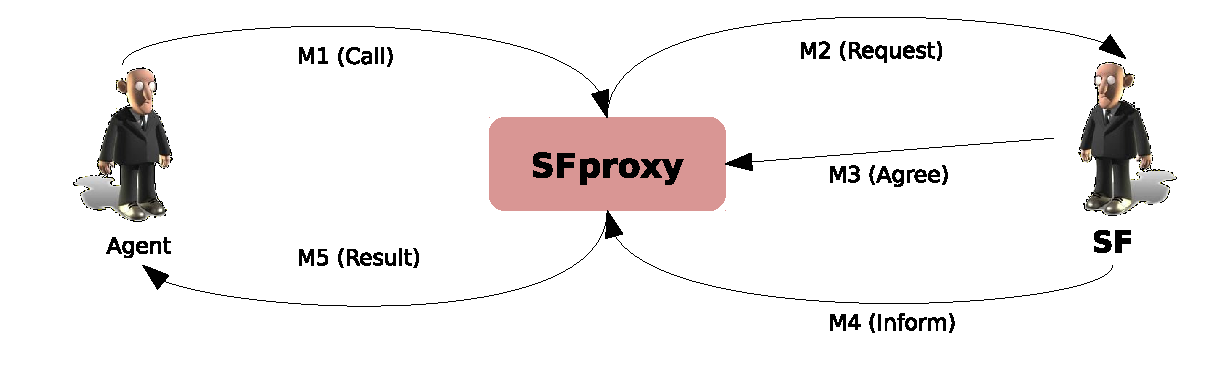
\includegraphics[width=1.0\textwidth]{Thomas/images/sf_sfProxy_interaction}
	\caption{Interaction between user agent and SF agent through the SFProxy}
\end{figure}


\subsubsection{Basic Service Management}
Services are composed by a profile, which is a semantic description of the  service, useful for customers to locate appropriate service, and a process, which details how to interact with the service.

Different agents can provide different processes (different implementations) to the same service profile (general description).

When an agent needs to register a new service in the organization, the \lstinline|RegisterService| method of the \lstinline|SFProxy| class is invoked. The following code shows how to register it in the organization.

\begin{lstlisting}

ArrayList<String> resultRegister= sfProxy.registerService("http://localhost:8080/testSFservices/testSFservices/owl/owls/Addition.owl");

\end{lstlisting}

\vspace{1cm}

The Register Service tries to register the service that is specified as parameter. The parameter is the original URL of the OWL-S specification of the service. The contents of the OWL-S specification of a service must have the profile that describes the service and the process that describes its implementation. If one or more providers (agents or organization) are specified in the \textit{profile:contactInformation} of the service, it means that the service is provided by agents or/and organizations. If there is one or more groundings, it means that the service is provided by a web service.


The Register Service returns a response describing if the service has been entirely registered or the number of providers and groundings added to an already registered service profile. In all cases, it returns a description of what is registered or not, and an OWL-S specification of the registered services or all data of the already registered service.



An agent can register its own implementation of an existing profile or create a new service from the scratch. In all cases, the OWL-S specification must have the profile and the process, and the Register Service will detect if the profile is already registered. In this case, the providers (agents, organizations, or groundings/web services) of the new specification will be added to the registered service in the SF database.


\subsubsection{Oracle: extracting information from OWL-S}
The Oracle is a class that allows developers to parse the profile of a semantic service, specified in OWL-S, in order to extract the required information (such as service inputs, outputs, providers, list of roles or organizational units).

Oracle needs just the OWL-S string containing the service specification to analyze it (as a parameter in the constructor of the class, see the example). This specification can be obtained with the method \lstinline|GetService| of the \lstinline|SFProxy| class.

Once the service specification is obtained, the oracle can be asked about any field in the service specification. The available methods for the Oracle class can be found in the Javadoc documentation of the project.

\begin{lstlisting}
//obtain the the service OWL-S specification
String serviceOWLS = sfProxy.getService(ServiceProfile);

//load in the oracle the service OWL-S specification and parse it
Oracle oracle = new Oracle(serviceOWLS);

//access to the service OWL-S information through the oracle
ArrayList<String> service_inputs = oracle.getOwlsProfileInputs();
ArrayList<Provider> providers = oracle.getProviders();
ArrayList<String> providersGroundingWSDL = oracle.getProvidersGroundingWSDL();
\end{lstlisting}





\section{Programming Agents that Offer Services}
This section describes how an agent that offers services to the other agents inside the organization can register, announce and provide its services.

%\subsection{Acquire Role}
%\begin{itemize}
%\item \textbf{Registration of an agent on the platform.} The agents request to be %registered as a \textit{participant} of the \textsc{Thomas} platform using the \lstinline|%AcquireRole| service:
%\begin{figure}[h!t]
%	\centering
%	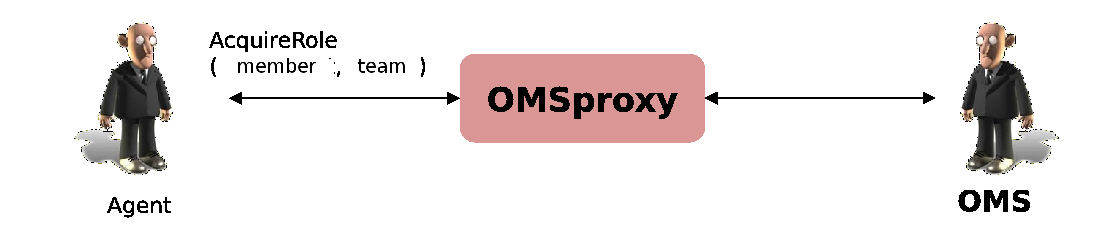
\includegraphics[width=.8\textwidth]{Thomas/images/acquireRoleparticipant}
%	\caption{Agent interaction protocol to acquire a role.}
%\end{figure}
%\begin{lstlisting}

%omsProxy.acquireRole("participant", "virtual");

%\end{lstlisting}


%\end{itemize}

\subsection{Service Registration}

\begin{itemize}
\item \textbf{Registering a new service}. An agent wants to register its own service in the SF (Figure \ref{fig:registerService}). The OWL-S specification of the service must be available in a url. This specification has to follow the OWL-S standard, having the profile and process of the service. It also needs to specify the provider or providers of the service in the following way:
\begin{itemize}
 \item If the provider is an agent or an organization,  the profile  has to be specified   as a \textit{provider} in the OWL-S specification. The provider is defined following the \textit{provider.owl} ontology, located in the \textit{webapps} folder of the Apache Tomcat in Magentix2 installation folder (concretely in \textit{webapps/ontologies}). The parameters of the provider are: entity id, entity type (agent or organization), communication language performative to use in the petition. An example of this structure is shown below:

 \begin{lstlisting}

  <profile:contactInformation>
    <provider:Provider rdf:ID="AdditionAgent">
	<provider:entityID rdf:datatype="^^xsd;string">AdditionAgent</provider:entityID>
	<provider:entityType rdf:datatype="^^xsd;string">Agent</provider:entityType>
	<provider:language rdf:datatype="^^xsd;string">FIPA-ACL</provider:language>
	<provider:performative rdf:datatype="^^xsd;string">REQUEST</provider:performative>
    </provider:Provider>
  </profile:contactInformation>

 \end{lstlisting}

 \item If the provider is a web service,  the corresponding grounding has to be specified  as standard specification of the OWL-S services including its WSDL document URL to execute the service.

\end{itemize}


\begin{figure}[h!t]
	\centering
	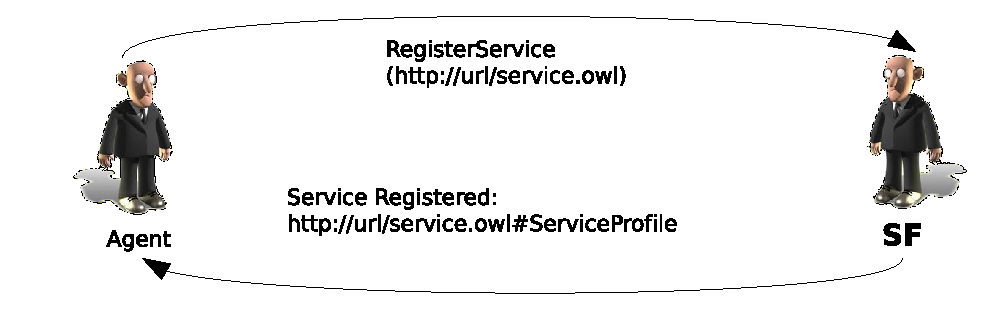
\includegraphics[width=.8\textwidth]{Thomas/images/registerService}
	\caption{Agent interaction protocol to register a service.}
	\label{fig:registerService}
\end{figure}

Thus, the agent can make a call to register a service specifying the url of the service OWL-S specification, as we can see in this code example:

\begin{lstlisting}

ArrayList<String> resultRegister = sfProxy.registerService("http://localhost:8080/testSFservices/testSFservices/owl/owls/Addition.owl");
\end{lstlisting}

\item \textbf{Registering new providers}. When a service is already registered, it is possible to add new providers (agents, organizations or web services). The \textit{RegisterService} of the SF detects automatically if the profile of the given OWL-S specification is already registered in the SF and just adds the new providers to the SF database. The given OWL-S specification must have the same profile so the SF recognize that is the same service and it associates the new providers to the registered service (see Figure \ref{fig:registerServiceProv}).

\begin{figure}[h!t]
	\centering
	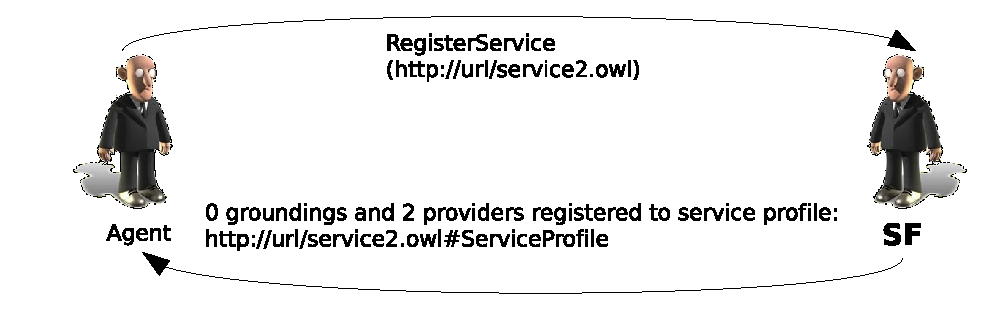
\includegraphics[width=.8\textwidth]{Thomas/images/registerServiceProv}
	\caption{Agent interaction protocol to register new providers.}
	\label{fig:registerServiceProv}
\end{figure}


\end{itemize}

\subsection{Provide services}
In \textsc{Thomas}, there are different ways of providing a service, as represented in Figure \ref{fig:handledServices}. On the one hand, in the cases that the providers are registered in the SF as agents or organizations, the requests to that services will be sent to the corresponding agent or organization as specified in the OWL-S registered in the SF. The agents or organizations can execute their service as an internal behaviour or as a web service, but this is not visible to the requester.

On the other hand, if the providers of a service are registered in the SF as web services (groundings), the requester of these services will have to execute the service by itself, using the class \textit{ServiceTools} of the package \textit{es.upv.dsic.gti\_ia.organization} (see Section \ref{sec:serviceRequestProcess}).



%\subsection{Execution of a Service} \label{sec:serviceExecution}
%If the provider of a service is a web service, the user has to execute it by itself. To perform this task, the class \textit{ServiceTools}  of the package \textit{es.upv.dsic.gti\_ia.organization} provides the method \textit{executeWebService} to facilitate the execution of web service to the developers. This method receives as parameters the url of the service WSDL document to execute it, and the inputs of the service. The inputs can be specified in two ways: in a \textit{HashMap} giving the name of the input and its value, or with an XML string in the following form:
%
%\begin{lstlisting}
% <inputs>
%  <inputX>valueX</inputX>
%  <inputY>valueY</inputY>
% </inputs>
%\end{lstlisting}
%
%Following we show an example to execute a web service (Square service of Thomas Example) in Magentix2 obtaining the OWL-S specification and the WSDL document of the service to execute.
%
%\begin{lstlisting}
%ArrayList<String> searchInputs=new ArrayList<String>();
%ArrayList<String> searchOutputs=new ArrayList<String>();
%ArrayList<String> searchKeywords=new ArrayList<String>();
%searchKeywords.add("squares");
%
%//search the service with some inputs, outputs and keywords
%ArrayList<ArrayList<String>> foundServices =
%sfProxy.searchService(searchInputs, searchOutputs, searchKeywords);
%//get the service OWL-S specification
%String serviceOWLS = sfProxy.getService(foundServices.get(0).get(0));
%
%//create an instance of the Oracle to obtain the service inputs and the WSDL url
%Oracle oracle = new Oracle(serviceOWLS);
%ArrayList<String> serviceInputs = oracle.getOwlsProfileInputs();
%ArrayList<String> providersGroundingWSDL = oracle.getProvidersGroundingWSDL();
%
%//fill the inputs with their names and values
%HashMap<String, String> agentInputs = new HashMap<String, String>();
%for (String input : serviceInputs) {
%  agentInputs.put(input, "35");
%}
%
%//execute the service and get the results in a HashMap
%HashMap<String, Object> resultExecution = st.executeWebService(providersGrounding.get(0), agentInputs);
%
%//get the final result of the service
%Double resultContent = (Double) resultExecution.get("Result");
%\end{lstlisting}





\section{Programming Agents that Request Services}
This section describes how an agent that requires services from other agents can search and request services in \textsc{Thomas}.

%\subsection{Acquire Role}
%\begin{itemize}
%\item \textbf{Registration of an agent on the platform.} The agents request to be %registered as a \textit{participant} of the \textsc{Thomas} platform using the \lstinline|%AcquireRole| service:
%\begin{figure}[h!t]
%	\centering
%	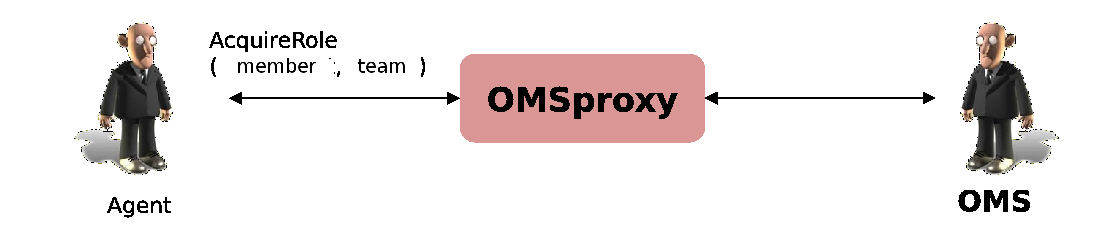
\includegraphics[width=.8\textwidth]{Thomas/images/acquireRoleparticipant}
%	\caption{Agent interaction protocol to acquire role.}
%\end{figure}
%\begin{lstlisting}
%omsProxy.acquireRole("participant", "virtual");
%\end{lstlisting}


%\end{itemize}


\subsection{Service Search Process}
\begin{itemize}
\item \textbf{Search of a service.} Agents can use the \lstinline|SearchService| service to find required services. The method \textit{SearchService} of the SFproxy makes a request to this service with the following parameters:
  \begin{itemize}
   \item List of inputs of the service to search. These inputs has to be specified as types of an ontology. In \textit{ServiceTools} class the main types (integer, float, double, string, boolean) are specified as constants to be easier to the developer.
   \item List of outputs of the service to search. These inputs has to be specified as types of an ontology, as the inputs explained before.
   \item List of keywords of the text description of the service to search. Each \textit{String} added to this list will compute to find it in the text description of the service profiles registered in the SF.
  \end{itemize}

\begin{figure}[h!t]
	\centering
	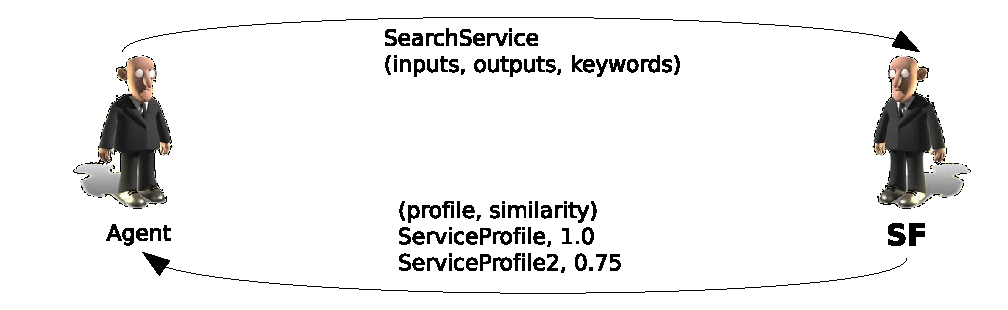
\includegraphics[width=.8\textwidth]{Thomas/images/searchService}
	\caption{Agent interaction protocol to search service.}
\end{figure}


The following example shows how to search for a service. The desired service should have the word "addition" in its description, two double inputs an one double output.

\begin{lstlisting}

ArrayList<String> searchInputs = new ArrayList<String>();
ArrayList<String> searchOutputs = new ArrayList<String>();
ArrayList<String> searchKeywords = new ArrayList<String>();

searchInputs.add(ServiceTools.OntologicalTypesConstants.DOUBLE);
searchInputs.add(ServiceTools.OntologicalTypesConstants.DOUBLE);

searchOutputs.add(ServiceTools.OntologicalTypesConstants.DOUBLE);

searchKeywords.add("addition");

ArrayList<ArrayList<String>> foundServices;

do {
	// Waiting for services
	try {
		Thread.sleep(2 * 1000);
	} catch (InterruptedException e) {

		e.printStackTrace();
	}
	foundServices = sfProxy.searchService(searchInputs, searchOutputs, searchKeywords);

} while (foundServices.isEmpty());



\end{lstlisting}
\end{itemize}


\subsection{Service Request Process}
\label{sec:serviceRequestProcess}

\begin{itemize}
\item \textbf{Request a service.} After the agent has found the desired service, it has to get the main information of this service to make a request. So the agent has to use the \textit{GetService} to obtain the required data to specify the inputs of the service and to know the provider to ask and its parameters. In the obtained OWL-S specification with \textit{GetService} is specified the providers of the service and their parameters. To make a request of the service, the provider has to be an agent or organization. In case that the providers are web services (with a grounding in the specification), the service has to be executed by the requester agent.

Using the \textit{Oracle} class provided in the package \textit{es.upv.dsic.gti\_ia.organization} the OWL-S specification is parsed to obtain the information of the service, including its inputs and its providers. There are two different ways to request a service depending on the type of the providers:
\begin{itemize}
 \item If the providers are \textbf{agents} or \textbf{organizations}, their parameters (entity ID, entity type, language and performative to make the request) are obtained from the OWL-S specification using the \textit{Oracle} class. Then, the requester agent should properly build the message to make the request and wait for the response of the provider to obtain the result. In \textit{ServiceTools} class it is possible to find the method \textit{buildServiceContent} which returns an XML description, receiving as parameters the inputs and the name of the requested service. This description is understood by all \textsc{Thomas} services and the services of the provided examples.

 \item If the providers are \textbf{web services}, the URL of the WSDL documents are obtained from the OWL-S specification using the \textit{Oracle} class. Then, the requester agent has to execute the service by itself. To perform this task, the class \textit{ServiceTools} of the package \textit{es.upv.dsic.gti\_ia.organization} provides the method \textit{executeWebService} to facilitate the execution of web services to the developers. This method receives as parameters  the url of the service WSDL document to execute it, and the inputs of the service. The inputs can be specified in two ways: in a \textit{HashMap} giving the name of the input and its value, or with an XML string in the following form:
  \begin{lstlisting}
   <inputs>
    <inputX>valueX</inputX>
    <inputY>valueY</inputY>
   </inputs>
  \end{lstlisting}
\end{itemize}

\end{itemize}

In the following example, the requester agent tries to make a request of the found service to the agent or organization providers if there are (providers list, lines 28-51). If there are not agent or organization providers (providers list is empty), then it tries to obtain the Web Services (groundings WSDL documents) that provide the service (providersGroundingWSDL list, lines 52-60). In this case, the requester agent has to execute the service by itself using the \textit{ServiceTools} class provided by \textsc{Thomas}.



\begin{lstlisting}
// Requesting the execution of the Addition service

// get the first service found because it is the most suitable
String serviceOWLS = sfProxy.getService(foundServices.get(0).get(0));

Oracle oracle = new Oracle(serviceOWLS);

// get service inputs
ArrayList<String> serviceInputs = oracle.getOwlsProfileInputs();

// put the service inputs values
HashMap<String, String> agentInputs = new HashMap<String, String>();

for (String input : serviceInputs) {
	if (input.equalsIgnoreCase("x"))
		agentInputs.put(input, "3");
	else if (input.equalsIgnoreCase("y"))
		agentInputs.put(input, "4");
	else
		agentInputs.put(input, "0");
}

// agents or organizations providers
ArrayList<Provider> providers = oracle.getProviders();
// web services providers
ArrayList<String> providersGroundingWSDL = oracle.getProvidersGroundingWSDL();

if (!providers.isEmpty()) {
	System.out.println("[" + this.getName() + "]" + " Requesting Addition Service (3+4)");

	// Building the ACL message
	ACLMessage msg = new ACLMessage();
	msg.setReceiver(new AgentID(providers.get(0).getEntityID()));
	msg.setLanguage(providers.get(0).getLanguage());
	msg.setPerformative(providers.get(0).getPerformative());
	msg.setSender(getAid());

  // Building the content of the message in XML
	String content = st.buildServiceContent(oracle.getServiceName(), agentInputs);

	// ACL message content is formed by XML format with service name
	// and
	// inputs
	msg.setContent(content);

	this.send_request(msg);

	ServiceTools st = new ServiceTools();
	HashMap<String, String> outputs = new HashMap<String, String>();
	st.extractServiceContent(requestResult, outputs);
	resultEquation = outputs.get("Result");
} else if (!providersGroundingWSDL.isEmpty()) {
	System.out.println("[" + this.getName() + "]" + " Executing Addition Service (3+4)");

	HashMap<String, Object> resultExecution = st.executeWebService(providersGroundingWSDL.get(0),
			agentInputs);

	Double resultDouble = (Double) resultExecution.get("Result");
	resultEquation = resultDouble.toString();
} else {// no providers for this service
	System.out.println("[" + this.getName() + "]" + " No providers found for Addition Service (3+4)");
}

\end{lstlisting}

\begin{figure}[h!t]
	\centering
	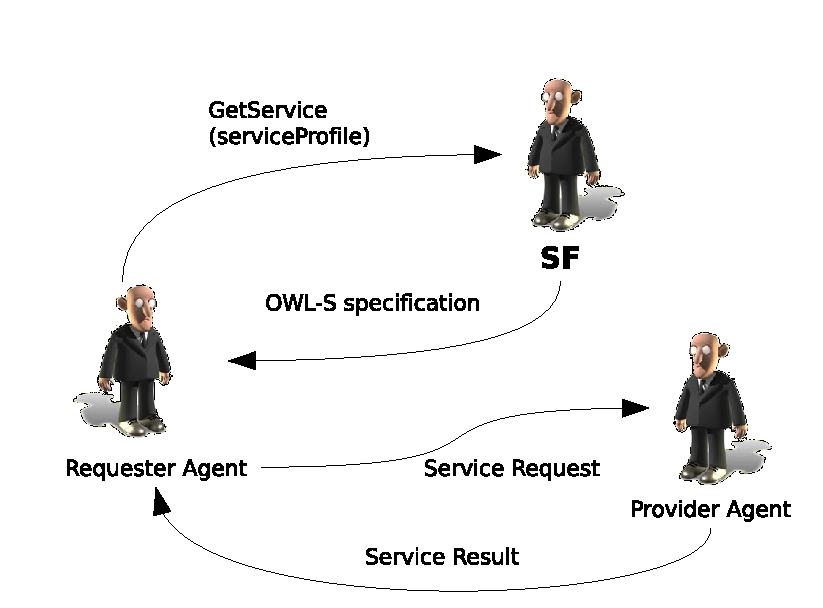
\includegraphics[width=.8\textwidth]{Thomas/images/serviceRequest}
	\caption{Agent interaction protocol to request a service.}
\end{figure}





%\begin{itemize}
%\item \textbf{Request a service.} After the agent has found the desired service, it has to get the main information of this service to make a request. So the agent has to use the \textit{GetService} to obtain the required data to specify the inputs of the service and to know the provider to ask and its parameters. In the obtained OWL-S specification with \textit{GetService} is specified the providers of the service and their parameters. To make a request of the service, the provider has to be an agent or organization. In case that the providers are web services (with a grounding in the specification), the service has to be executed by the requester agent (see Section \ref{sec:serviceExecution}). Using the \textit{Oracle} class provided in the package \textit{es.upv.dsic.gti\_ia.organization} the OWL-S specification is parsed to obtain the information of the service, including its inputs and its providers with their corresponding parameters. Taking the entity id of the provider to ask, its language and its performative, the requester agent can build the message to make the request. Finally, the requester has to wait for the response of the provider and obtain the result.
%
%In the following example, the requester agent tries to make a request of the found service to the agent or organization providers if there are (providers list). If there are not agent or organization providers (providers list is empty), then it tries to obtain the Web Services (groundings WSDL documents) that provide the service (providersGroundingWSDL list). In this case, the requester agent has to execute the service by itself using the \textit{ServiceTools} class provided by \textsc{Thomas}.
%\begin{lstlisting}
%
%
%// Requesting the execution of the Addition service
%
%// get the first service found because it is the most suitable
%String serviceOWLS = sfProxy.getService(foundServices.get(0).get(0));
%
%Oracle oracle = new Oracle(serviceOWLS);
%
%// get service inputs
%ArrayList<String> serviceInputs = oracle.getOwlsProfileInputs();
%
%// put the service inputs values
%HashMap<String, String> agentInputs = new HashMap<String, String>();
%
%for (String input : serviceInputs) {
%	if (input.equalsIgnoreCase("x"))
%		agentInputs.put(input, "3");
%	else if (input.equalsIgnoreCase("y"))
%		agentInputs.put(input, "4");
%	else
%		agentInputs.put(input, "0");
%}
%
%// agents or organizations providers
%ArrayList<Provider> providers = oracle.getProviders();
%// web services providers
%ArrayList<String> providersGroundingWSDL = oracle.getProvidersGroundingWSDL();
%
%if (!providers.isEmpty()) {
%	System.out.println("[" + this.getName() + "]" + " Requesting Addition Service (3+4)");
%
%	// Building the ACL message
%	ACLMessage msg = new ACLMessage(ACLMessage.REQUEST);
%	msg.setReceiver(new AgentID(providers.get(0).getEntityID()));
%	msg.setProtocol("fipa-request");
%	msg.setSender(getAid());
%
%	String content = st.buildServiceContent(oracle.getServiceName(), agentInputs);
%
%	// ACL message content is formed by XML format with service name
%	// and
%	// inputs
%	msg.setContent(content);
%
%	this.send_request(msg);
%
%	ServiceTools st = new ServiceTools();
%	HashMap<String, String> outputs = new HashMap<String, String>();
%	st.extractServiceContent(requestResult, outputs);
%	resultEquation = outputs.get("Result");
%} else if (!providersGroundingWSDL.isEmpty()) {
%	System.out.println("[" + this.getName() + "]" + " Executing Addition Service (3+4)");
%
%	HashMap<String, Object> resultExecution = st.executeWebService(providersGroundingWSDL.get(0),
%			agentInputs);
%
%	Double resultDouble = (Double) resultExecution.get("Result");
%	resultEquation = resultDouble.toString();
%} else {// no providers for this service
%	System.out.println("[" + this.getName() + "]" + " No providers found for Addition Service (3+4)");
%}
%
%\end{lstlisting}
%
%\begin{figure}[h!t]
%	\centering
%	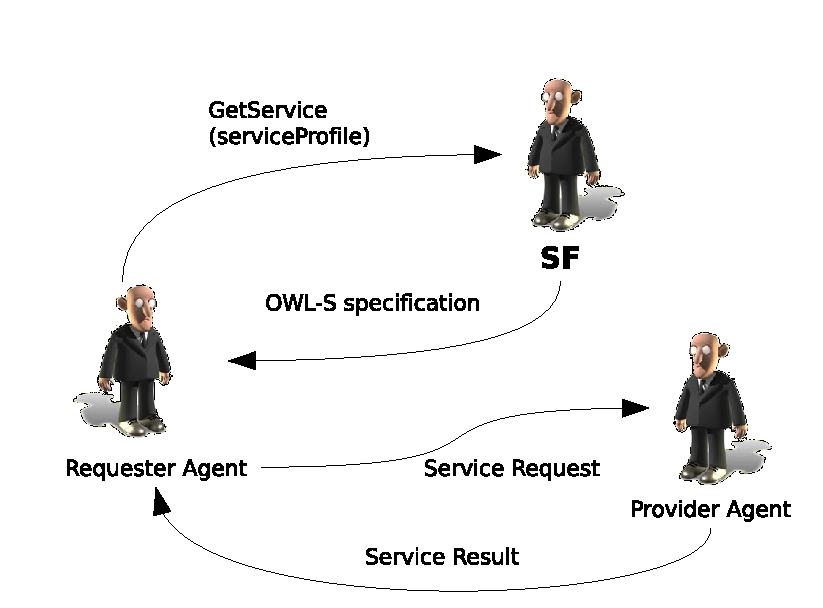
\includegraphics[width=.8\textwidth]{Thomas/images/serviceRequest}
%	\caption{Agent interaction protocol to request a service.}
%\end{figure}
%
%\end{itemize}






\section{Running \textsc{Thomas} Example}

The examples folder of the Magentix2 packages contains a basic \textsc{Thomas} example. In this example there are four agents:
\begin{itemize}
 \item \textbf{Initiator}. This agent build the organizational framework needed. First, it registers the \textit{Calculator} and \textit{School} organizations. Then, it registers the roles needed in each organization. As this agent register each unit, it also plays the role \textit{Creator} of them. At the end of the example, it deallocates all roles and deregister all units, roles and services.
 \item \textbf{Addition}. This agent acquires the role \textit{Operation} of the \textit{Calculator} organization. It also registers and provides the service \textit{Addition}.
 \item \textbf{Product}. This agent acquires the role \textit{Operation} of the \textit{Calculator} organization. It also registers the services \textit{Product} and \textit{Square}. It only provides the service \textit{Product}.
 \item \textbf{James}. It represents an student which needs computing some operations and demand the other their services. This agent acquires the role \textit{Student} of the \textit{School} organizations. It looks for the different services it needs (Addition, Product and Square) to calculate a simple mathematical operation. Then either ask the service providers in carrying out such services, or run them directly if no provider.
\end{itemize}

Services in the \textsc{Thomas} example are deployed in the \textit{webapps} folder of the Apache Tomcat in Magentix2 installation folder. The OWL-S specifications are located in:
\begin{lstlisting}
webapps/testSFservices/testSFservices/owl/owls/
\end{lstlisting}
The WSDL documents can be found in:
\begin{lstlisting}
 webapps/testSFservices/WEB-INF/services/service_name/META-INF/service_name.wsdl
\end{lstlisting}

The following services are used in the \textsc{Thomas} example:
\begin{itemize}
 \item \textbf{Product}: This service multiplies two input numbers (doubles) and returns the product (double). It is provided by an agent behavior.
 \item \textbf{Addition}: This service adds two input numbers (doubles) and returns the addition (double). It is provided by agent that calls to a web service.
 \item \textbf{Square}: This service squares an input number (double) and returns the result (double). It is provided by a web service.
\end{itemize}

Following, we briefly explain the actions of the \textsc{Thomas} example shown in the diagram of Figure \ref{fig:ThomasExample}:

\begin{figure}[h!t]
	\centering
	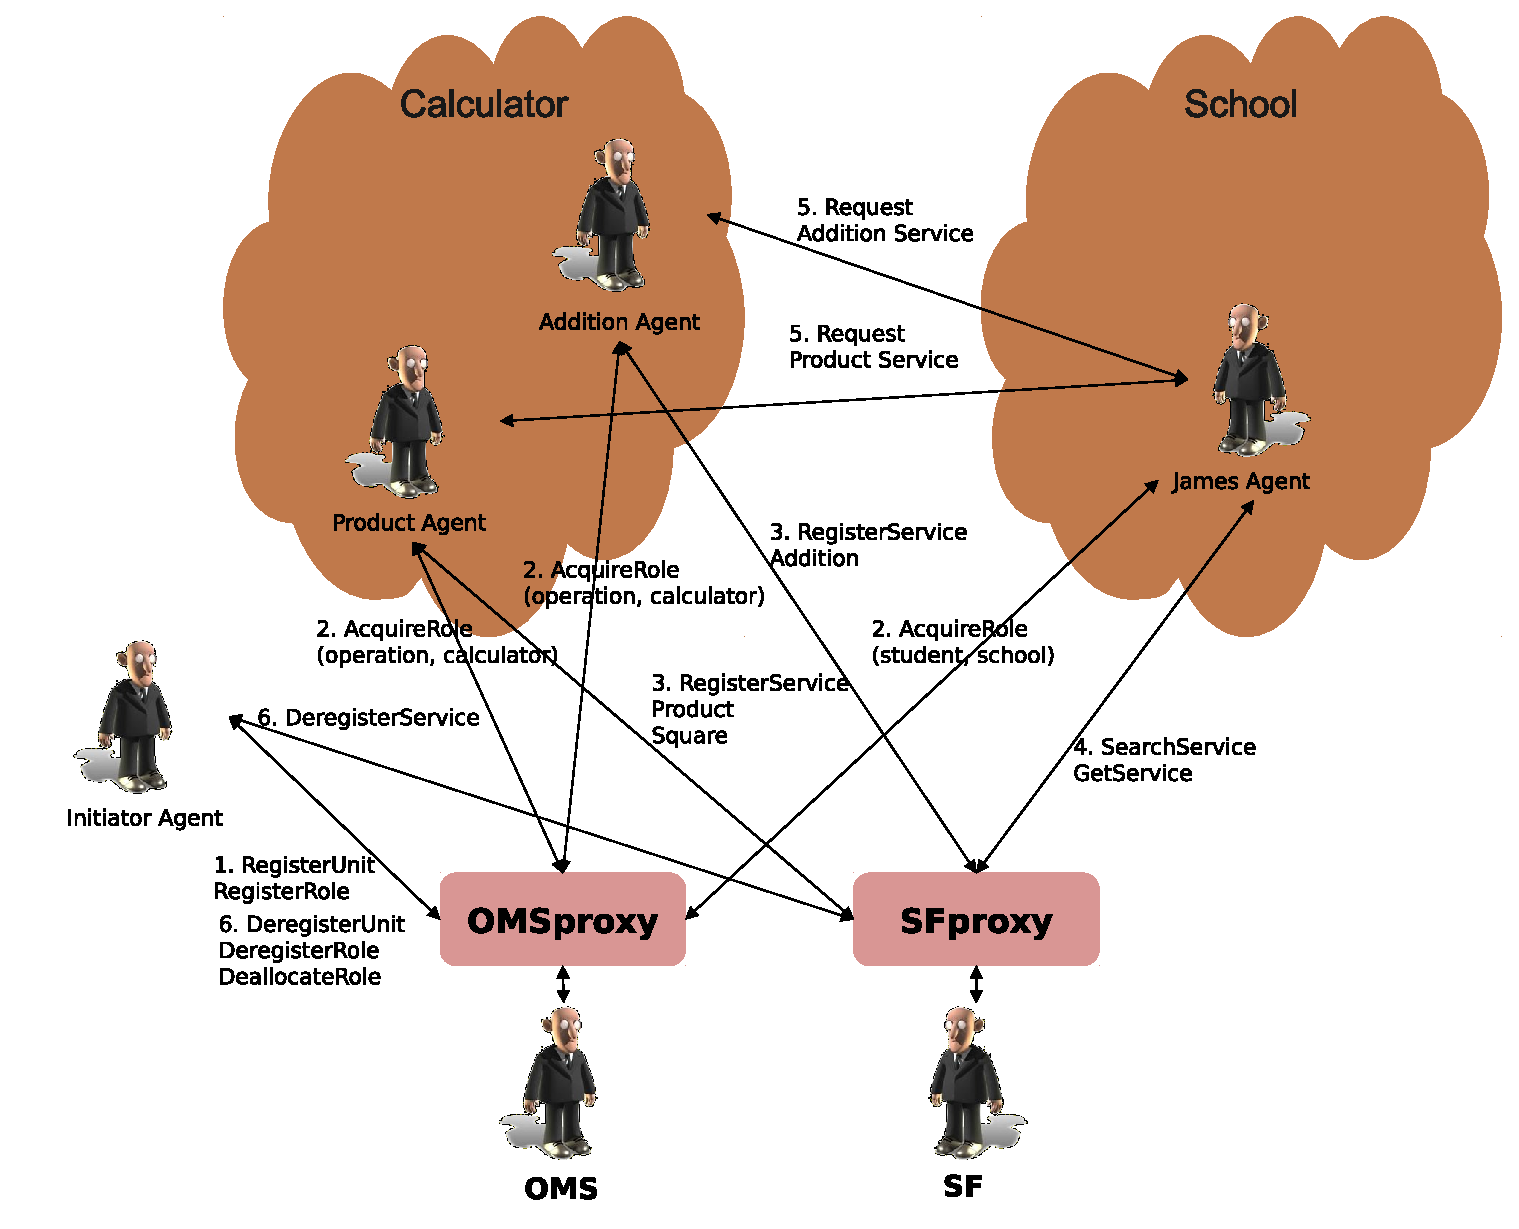
\includegraphics[width=1\textwidth]{Thomas/images/thomasExample}
	\caption{Thomas Example diagram}
	\label{fig:ThomasExample}
\end{figure}

\begin{enumerate}
 \item The Initiator acquires the role \textit{participant} of the default unit \textit{virtual}. Then, it registers the organizations \textit{Calculator} and \textit{School}. \textit{Calculator} is a team unit, its parent unit is virtual and the name of the default role is \textit{creator}. On the other hand, the unit \textit{School} is a flat organization, its parent unit is virtual and the name of the default role is also \textit{creator}. Once the agent registers the units, it also creates the roles needed. So, first the Initiator agent registers a role named \textit{operator} (member, public and external) inside the unit \textit{Calculator}. Secondly, it registers a role named \textit{student} (member, public and external) inside the unit \textit{School}.

 \item The Addition agent and the Product agent acquire the role \textit{operation} of the \textit{Calculator} organization. Also, the James agents acquires the role \textit{student} of the \textit{School} organization.

 \item The Addition agent registers the Addition service in the SF. Also, the Product agent registers the Product and Square services in the SF.

 \item The James agent wants to calculate the equation $(5 (3 + 4))^2$. Firstly, it searches for a service to add two numbers and it finds the Addition service. It makes a \textit{GetService} of this service to obtain the required information to request it. It also searches for a service to make the product and another one to square. In these cases, it finds the Product service and the Square service. It makes a \textit{GetService} of the two services to obtain their information.

 \item The James agent requests the Addition service to add 3 and 4. Then, with this result requests the Product service to multiply it by 5. Finally, the result of this operation is used to square it with the Square service, that is provided by a web service. This implies that the James agent has to execute it itself by using the Service Tools provided in the Magentix2 API. The James agent has obtained the final result of the equation that it wanted to solve. Then, it sends a message to the Initiator agent to inform that the example has ended.

 \item The Initiator agent receives the message informing that the example has ended. It deallocates all the roles and deregisters all services, roles and units.

\end{enumerate}

To run the example the user has to enter in the Magentix2/examples folder where it has been installed. Then, the user has to execute the \textit{Start-ThomasExample.sh} script with administrator privileges:

\begin{lstlisting}
cd Magentix2/examples/bin/
sudo sh Start-ThomasExample.sh
\end{lstlisting}


\section{Programming agents which use organizational messaging}



This section describes how an agent that wants to send a message to an organization
can build, fill the fields of an ACLMessage and send the organizational message.
The example shown in Figure \ref{fig:org1}  is used to illustrate this section. It is formed by: the \textit{Sender Agent} that acquires role member in the unit \textit{team} and two \textit{Receivers Agents} with the role member in the unit team ). The unit virtual is parent of the unit \textit{team}.

\begin{figure}[h!t]
	\centering
	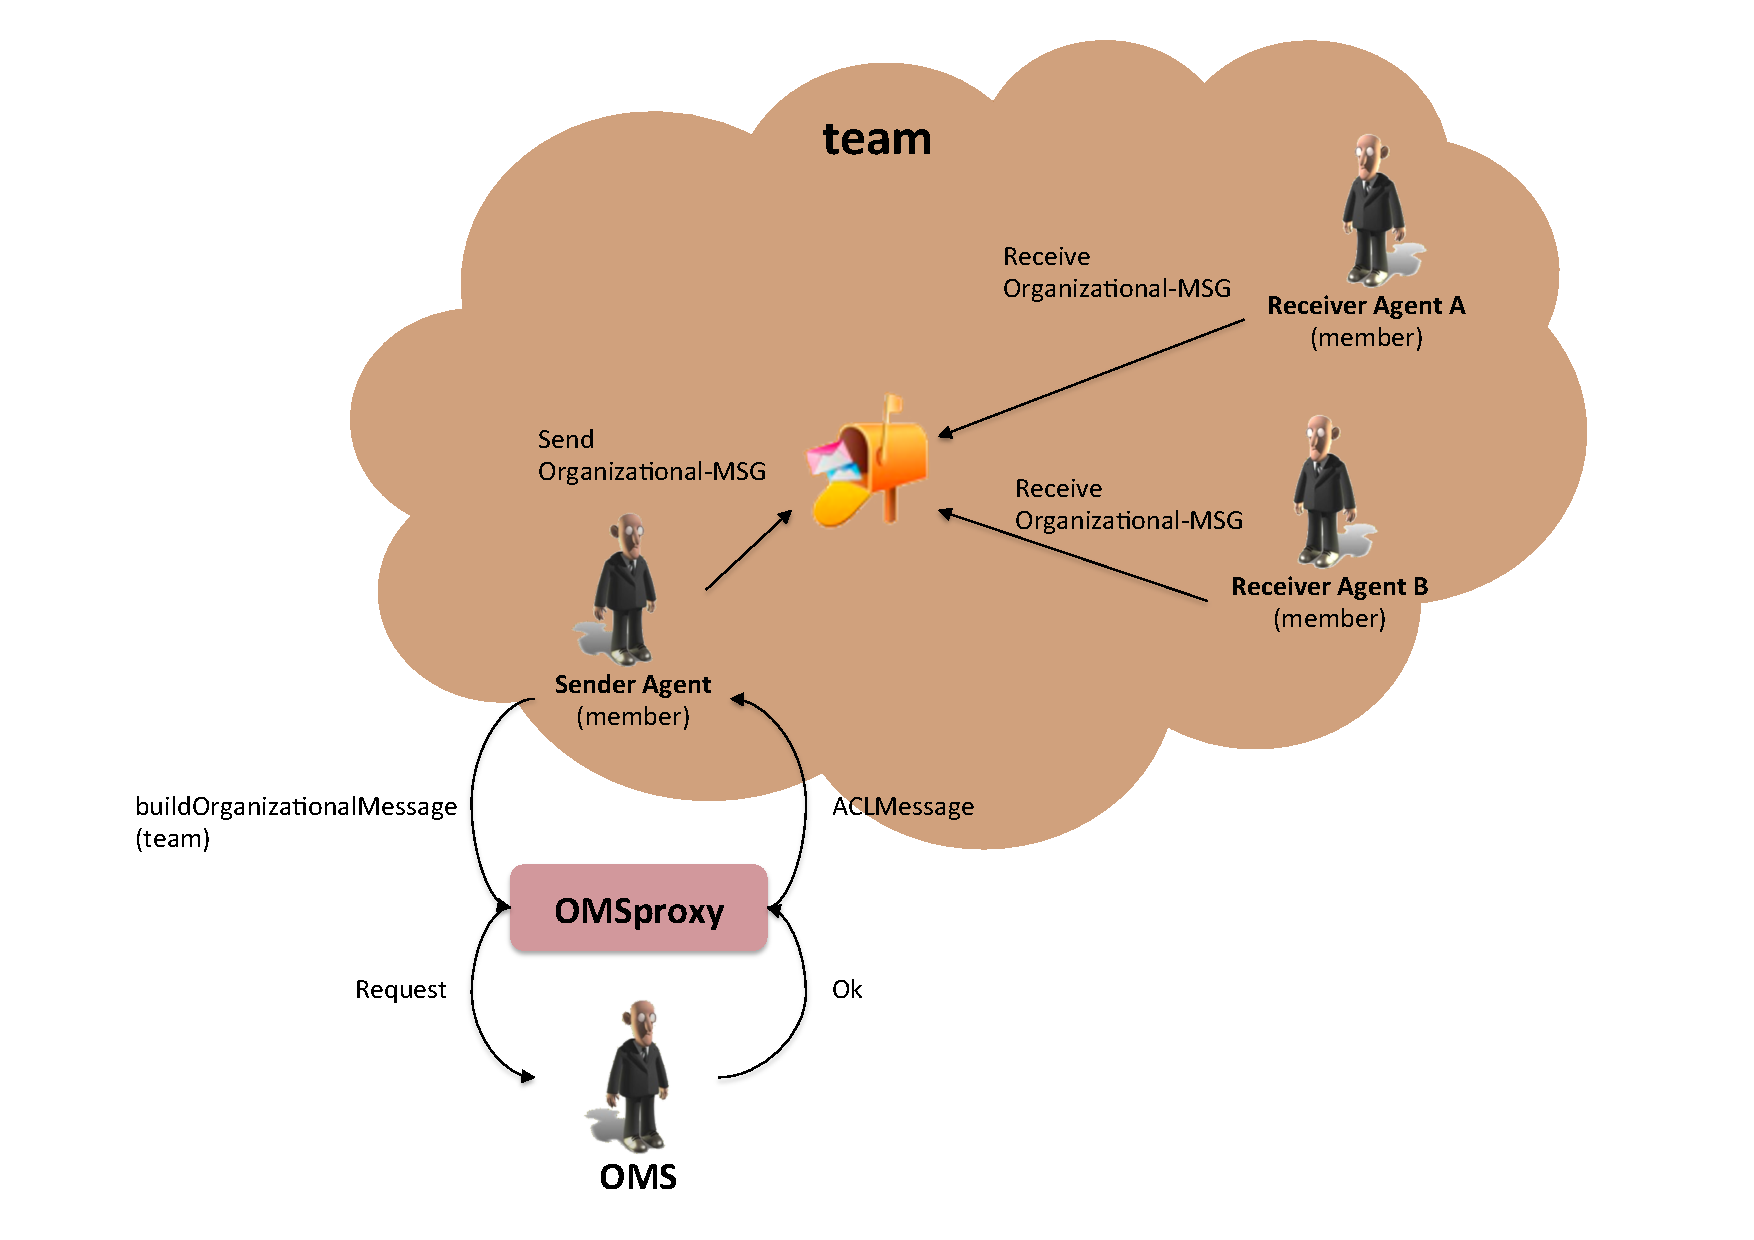
\includegraphics[width=1\textwidth]{Thomas/images/org.pdf}
	\caption{Organizational messaging: Example diagram.}
	\label{fig:org1}
\end{figure}


\subsection{Registration into the organization}


\begin{figure}[h!t]
	\centering
	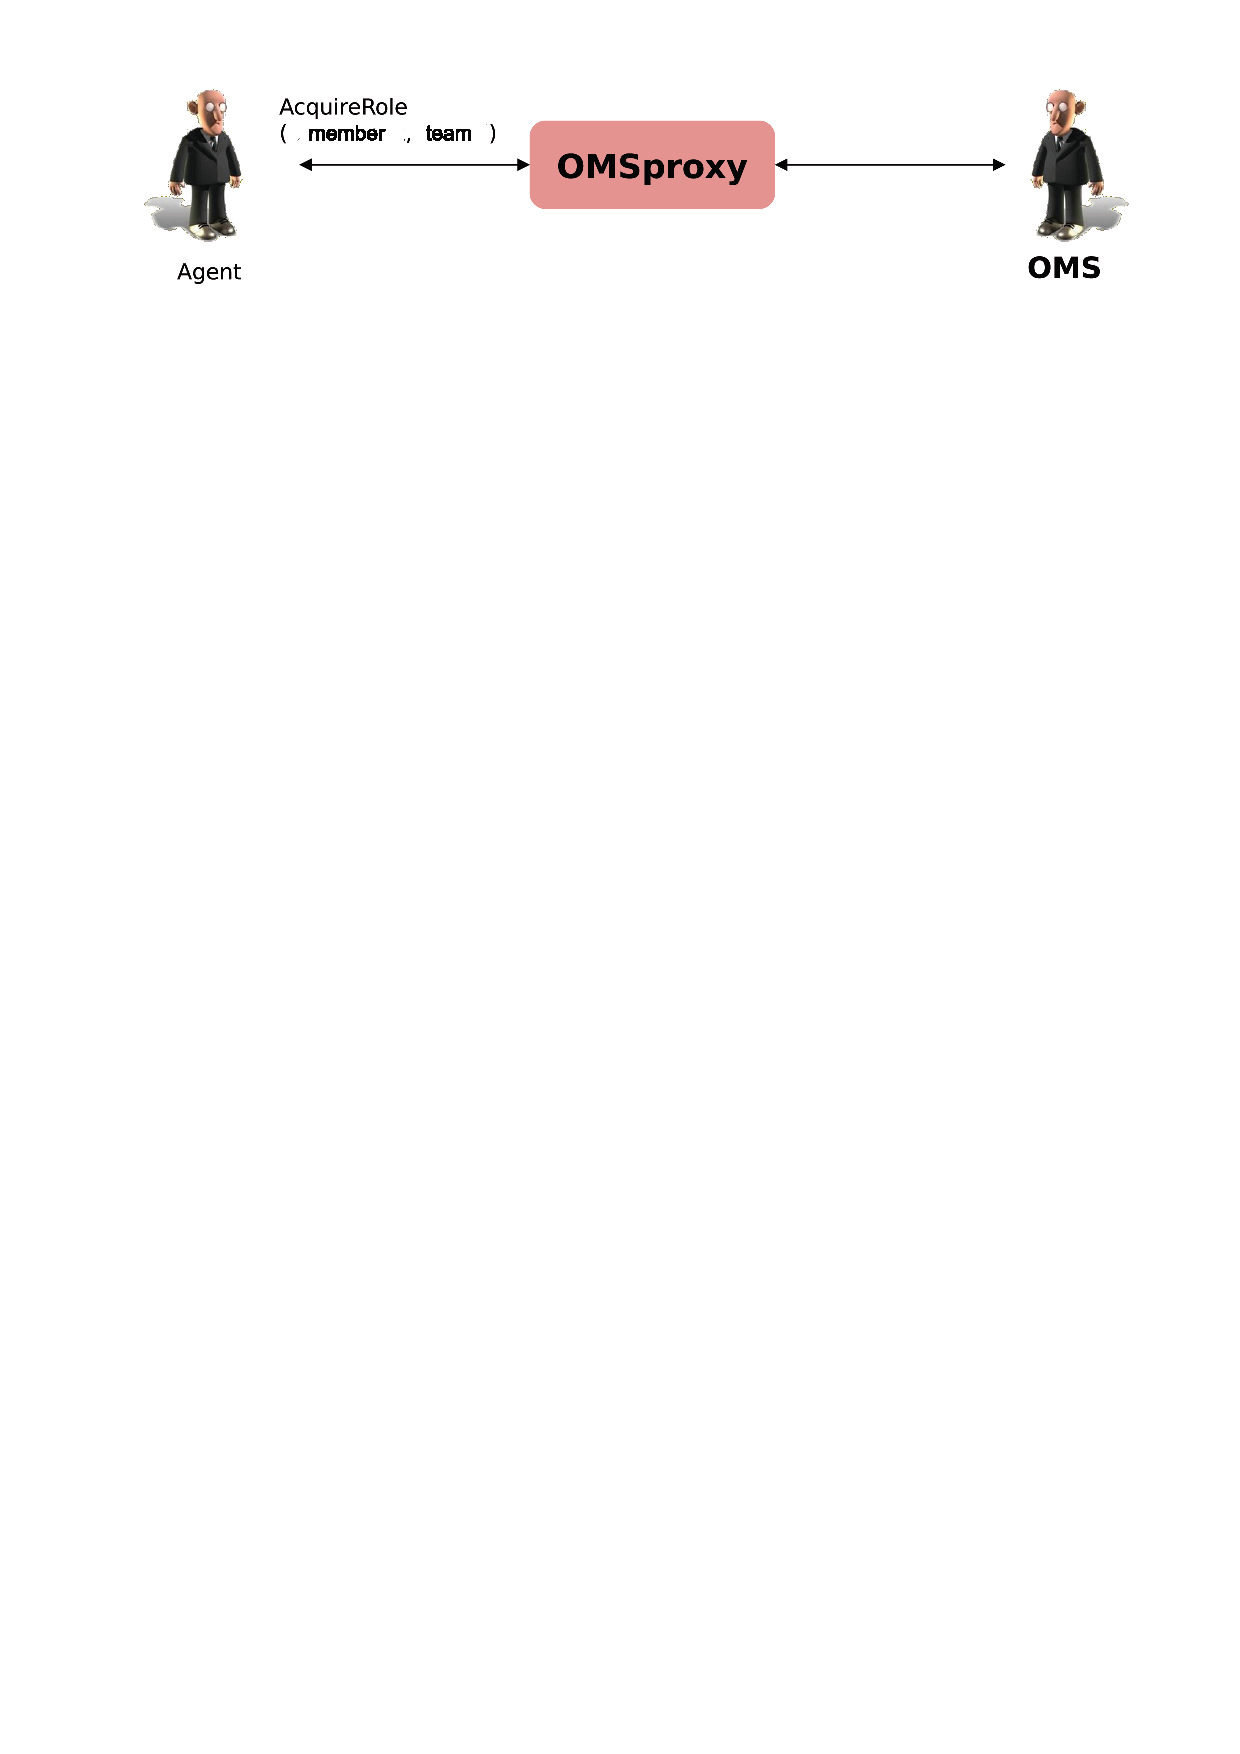
\includegraphics[width=.8\textwidth]{Thomas/images/acquireRoleMember}
	\caption{Agent interaction protocol to acquire role.} \label{fig:agentAcquireRole}
\end{figure}

\begin{itemize}
\item \textbf{Registration in the unit.} Agents need to be registered into the organizations by means of acquiring some available role before using organizational messaging. For example, in figure \ref{fig:org1}, an organization called \textit{team} is shown. In this organization the role \textit{member} is available. Thus, the\textit{ Sender Agent} should play the role member before sending an organizational message to the \textit{Receiver Agents A} and \textit{B}. If it does not play the required role, it should acquire it by means of the AcquireRole service (figure \ref{fig:agentAcquireRole}). 




\begin{lstlisting}

omsProxy.acquireRole("member", "team");

\end{lstlisting}

\end{itemize}
\subsection{Building the Message}
\begin{itemize}
\item \textbf{Build an organizational message.} Once the agent is inside the unit with an specific role, it has to use the \textit{buildOrganizationalMessage} to
obtain the required organizational message specifying the identifier of the organization:
\begin{lstlisting}
ACLMessage msg = omsProxy.buildOrganizationalMessage("team");
\end{lstlisting}
\end{itemize}

\subsection{Completing Message}
\begin{itemize}
\item \textbf{Add ACL message fields.} After the message is built, it can add the fields of an ACLMessage, such as content, performative or language:
\begin{lstlisting}
msg.setContent(6+" "+3);
msg.setPerformative(ACLMessage.REQUEST);
msg.setLanguage("ACL");
\end{lstlisting}
\end{itemize}
\subsection{Sending the Message}
\begin{itemize}
\item \textbf{Send an organizational message.} When a message is formed,the message can be sent  using the \textit{send()} method:

\begin{lstlisting}
send(msg);
\end{lstlisting}
or it reached a state of type send in CFactories:
\begin{lstlisting}
class REQUEST_Method implements SendStateMethod {


  public String run(CProcessor myProcessor, ACLMessage messageToSend) {


    OMSProxy omsProxy = new OMSProxy(myProcessor);
    ACLMessage msg;
    String state = "WAIT";
    try {
	msg = omsProxy.buildOrganizationalMessage("team");
	messageToSend.copyFromAsTemplate(msg);

	messageToSend.setPerformative(ACLMessage.REQUEST);
	messageToSend.setLanguage("ACL");
	messageToSend.setContent(6+" "+3);

    } catch (THOMASException e) {
	e.printStackTrace();
	state="FINAL";
    }
    return state;
  }
}
\end{lstlisting}
\end{itemize}

\section{Organizational Messaging Example}

The examples folder of the Magentix2 packages contains an Organizational Message example. This example shows an scenario with THOMAS organizations and CAgents that make use of organizational messaging. This case consists of the following two units:

\begin{itemize}
\item \textbf{Calculator:} \textit{Team} type organization where its agents send Organizational Messages to
  calculate the sum of the transaction carried out by its agents.
\item \textbf{External:} \textit{Flat} type organization whose unique purpose is that one of its agents
  tries to send a Organizational Message to \textit{Calculator} organization.
\end{itemize}

The agents involved in this case and its features are described below:

\begin{itemize}
\item \textbf{Creator:} Agent who plays the \textit{Creator} role with \textit{creator} position within
  \textit{Calculator} organization, whose purpose will be to create the entire organizational structure
  (organization and roles). In addition, it tries to send an Organizational Message to the \textit{Calculator}
  organization, requesting some calculation using two numbers.
\item \textbf{Display:} Agent who plays the \textit{Manager} role with \textit{member} position within
  \textit{Calculator} organization, whose unique purpose is sending console messages to inform about messages
  sent by agents with \textit{Manager} role within \textit{Calculator} organization.
\item \textbf{Summation:} Agent who plays the \textit{Manager} role with \textit{member} position within
  \textit{Calculator} organization. It requests to each of its subordinates to do the operation for which
  they are prepared. Then, it adds up all the responses and sends a message reporting the result.
\item \textbf{Product:} Agent who plays the \textit{Operator} role with \textit{member} position within
  \textit{Calculator} organization. It only provides the Product operation and informs of the result.
\item \textbf{Addition:} Agent who plays the \textit{Operator} role with \textit{member} position within
  \textit{Calculator} organization. It only provides the Addition operation and informs of the result.
\item \textbf{Noisy:} Agent who plays two roles. The first, the \textit{Creator} role with \textit{creator}
  position within \textit{External} organization as a result to create this organization. The second, the
  \textit{Manager} role with \textit{member} position within \textit{External} organization. It tries to send
  a Organizational Message to the \textit{Calculator} organization, requesting a calculation using two
  numbers.
\end{itemize}

Following, we briefly explain the actions of the Organizational Message example shown in the diagram of Figure \ref{fig:OMessageDiagram}:

\begin{figure}[h!t]
	\centering
	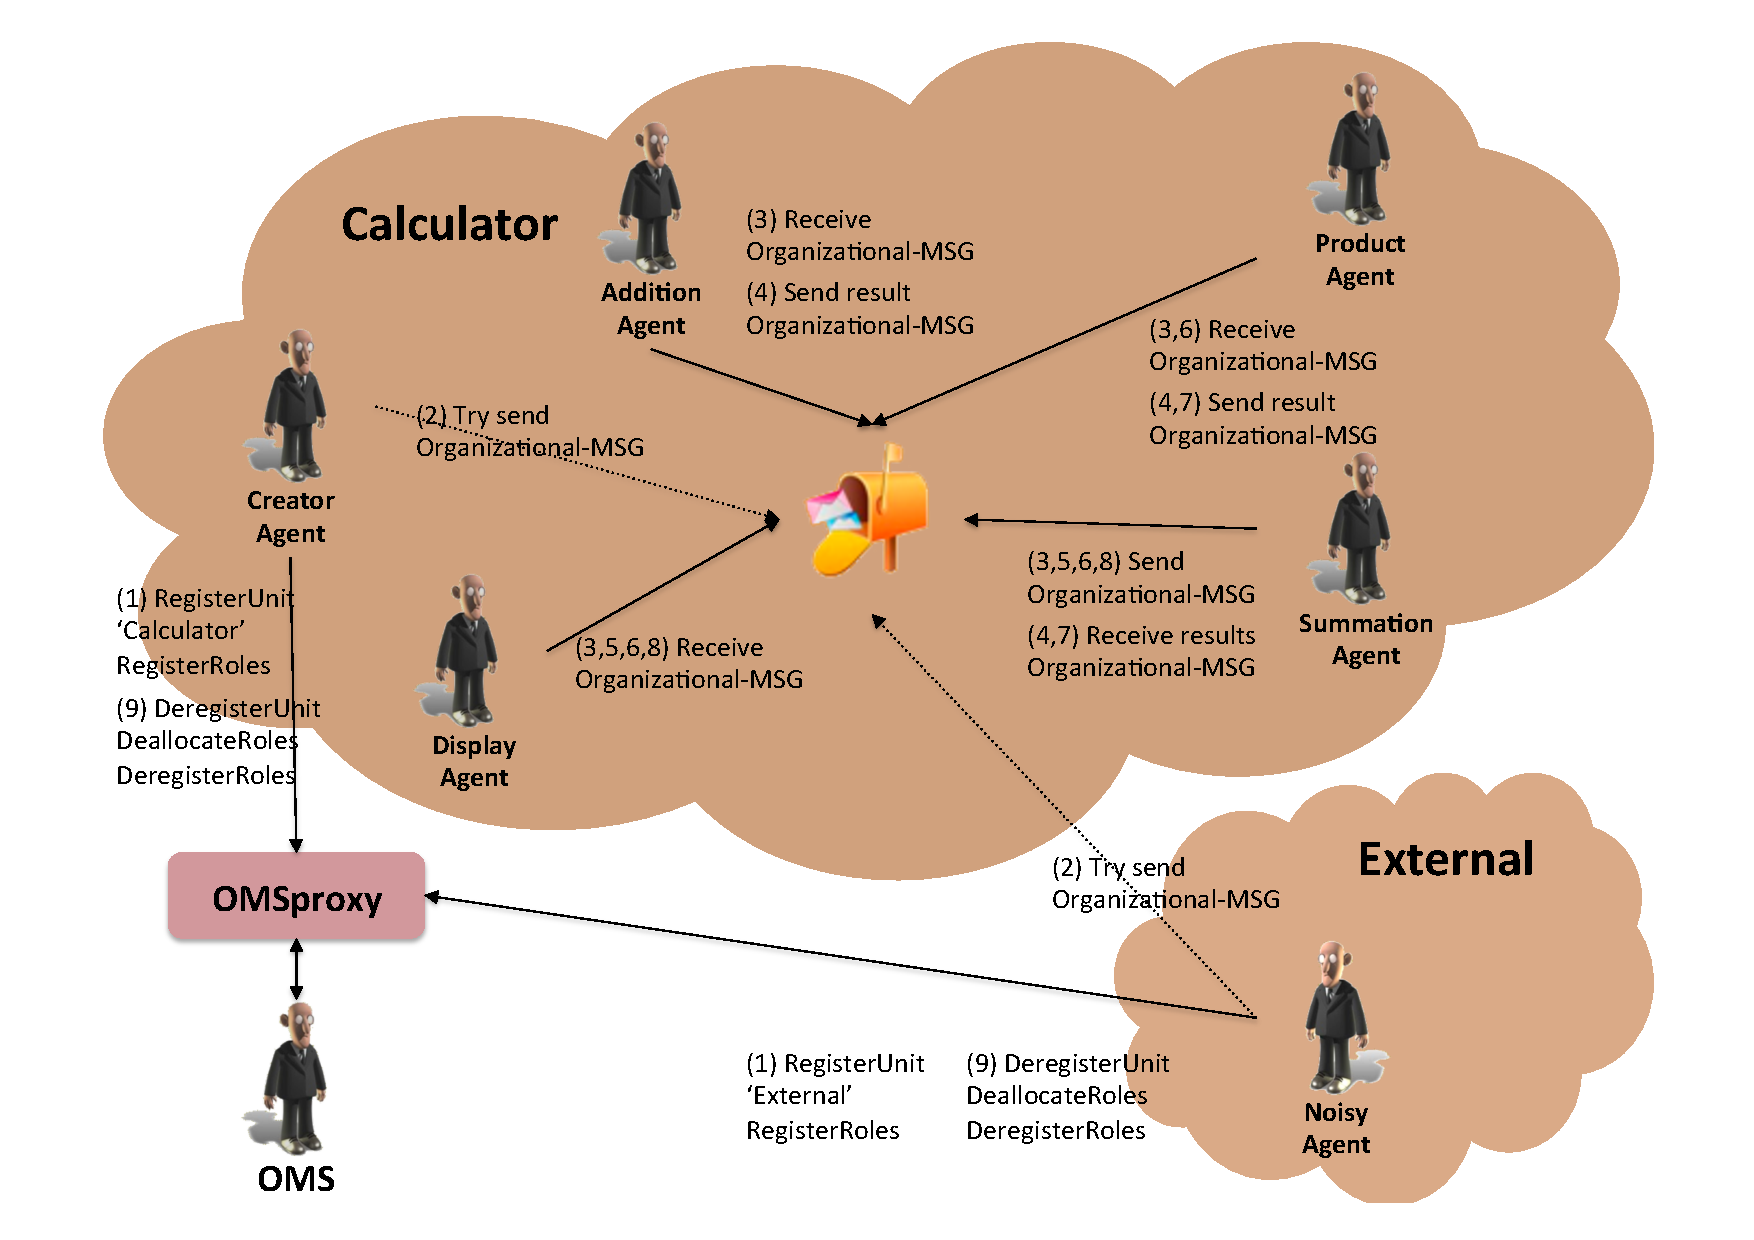
\includegraphics[width=\textwidth]{Thomas/images/organizationalMessageExample}
	\caption{Organizational Message Example diagram}
  \label{fig:OMessageDiagram}
\end{figure}

\begin{enumerate}
\item Scenario creation is the first task to begin the example. The Creator agent creates the \textit{Calculator}   organization and their roles (\textit{Creator},\textit{Manager} and \textit{Operator}). Simultaneously,   the Noisy agent creates the \textit{External} organization and their roles (\textit{Creator} and \textit{Manager}). All agents begin its execution in the scenario.
\item The Creator and Noisy agents try to build an organizational message but their requests are rejected.   The Creator agent can not send an organizational message because it only plays the \textit{Creator}
  role with \textit{creator} position within \textit{Calculator} organization. In the same way, the Noisy
  agent can not send an organizational message because it doesn't belong to \textit{Calculator} organization.
\item The Summation agent sends Formula(6,3) as an organizational message. This is received by the Product,
  Addition and Display agents. The Display agent prints this message to standard output.
\item The agents that play the \textit{Operator} role (Addition and Product agents) receive the numbers
  (six and three) to calculate their calculations ($6+3=9$ and $6*3=18$, respectively) and communicate
  the results as an organizational messages. These are received by the Summation agent. The Addition agent
  leaves the \textit{Operator} role.
\item The Summation agent sends the sum of all results received ($9+18=27$) as an organizational message.
  This is received by the Display agent, which prints this value to standard output.
\item The Summation agent sends Formula(5,3) as an organizational message. This is received by the Product
  and Display agents. The Display agent prints this message to standard output.
\item The agents that play the \textit{Operator} role (only Product agent) receive the numbers (five and three)
  to calculate their calculations ($5*3=15$) and communicate the results as an organizational messages. These
  are received by the Summation agent.
\item The Summation agent sends the sum of all results received ($15=15$) as an organizational message. This
  is received by the Display agent, which prints this value to standard output.
\item To finalize this example, the scenary is disassembled. The Creator agent deregisters all the roles belonging to \textit{Calculator} organization and deregisters the organization. Simultaneously,
  the Noisy agent deallocates and deregisters all the roles belonging to the \textit{External} organization and
  deregisters the organization. All agents finalize their executions.
\end{enumerate}

To run the example the user has to enter in the Magentix2/examples/bin folder where it has been installed. Then,
the user has to execute the Start-OrganizationalExample.sh script with administrator privileges:

\begin{lstlisting}
cd Magentix2/examples/bin/
sudo sh Start-OrganizationalExample.sh
\end{lstlisting}
 
